% AnchorMTM with updated correspondence and Storms teaser, 2026-11-02.
% Build: tectonic -X compile --keep-logs method_anchor_figures_updated_en.tex
% Unchanged companion: method_anchor_single_parameter_supplement.tex/.pdf.
% Changes: ANCHORMTM_SINGLE_PARAMETER_VALIDATION.md.
\documentclass[review]{vgtc}
\usepackage[T1]{fontenc}
\usepackage{mathptmx}
\usepackage{cite}
\usepackage{amsmath,amssymb,amsthm}
\usepackage{placeins}
\usepackage{booktabs,multirow,colortbl}
\makeatletter
\setlength{\@dblfptop}{0pt}
\setlength{\@dblfpsep}{12pt}
\setlength{\@dblfpbot}{0pt plus 1fil}
\makeatother
\usepackage[ruled,vlined]{algorithm2e}
\SetKwInput{KwData}{Data}
\SetKwInput{KwResult}{Result}
\SetKwProg{Fn}{Function}{:}{}
\SetKw{KwReturn}{return}
\SetKw{KwBreak}{break}
\SetKwFunction{Construct}{ConstructTemporalMap}
\SetKwFunction{Refine}{RefineOrder}
\SetKwFunction{Barriers}{OptimalBarriers}
\SetAlFnt{\small}
\SetAlCapFnt{\small\bfseries}
\SetAlCapNameFnt{\small\bfseries}
\SetAlCapSkip{3pt}
\DontPrintSemicolon
\setcounter{secnumdepth}{3}
\newtheorem{theorem}{Theorem}
\newtheorem{lemma}{Lemma}
\newtheorem{proposition}{Proposition}
\newcommand{\dtop}{d_{\mathrm{top}}}
\newcommand{\lca}{\operatorname{lca}}
\newcommand{\nroe}{\mathrm{NROE}}
\newcommand{\pos}[1]{\left[#1\right]^+}
\title{AnchorMTM: Spatially Anchored Merge Tree Maps\\for Time-Varying Scalar Fields}
\author{Anonymous Authors}
\onlineid{0}
\vgtccategory{Research}
\vgtcinsertpkg
\hypersetup{pdftitle={AnchorMTM: Spatially Anchored Merge Tree Maps for Time-Varying Scalar Fields},pdfauthor={Anonymous Authors}}
\abstract{Temporal merge tree maps preserve evolving scalar hierarchies, but their display axis need not carry a fixed spatial meaning. How much reference displacement is forced by the hierarchy, and how much comes from the layout? We derive three algorithm-independent bounds for exact-topology point orders, finite-width interval layouts, and layouts with bounded merge-level error. The point bound is attainable and separates unavoidable order error from excess introduced by the ordering rule; the width-aware bounds certify displacement without assuming a particular objective or solver. AnchorMTM uses a shared spatial reference, topology-budgeted order search, capped anchor placement and scalar-profile reconstruction to construct such maps. Existing planar and volumetric comparisons document reference alignment, relative geometry and achieved topology error separately. The results support a controlled position--topology trade-off: a hierarchy imposes quantifiable conflicts with a spatial axis, rather than excluding that axis altogether.}
\keywords{Time-varying scalar fields, merge tree maps, spatial anchoring, topology preservation, constrained layout.}
\teaser{
\centering
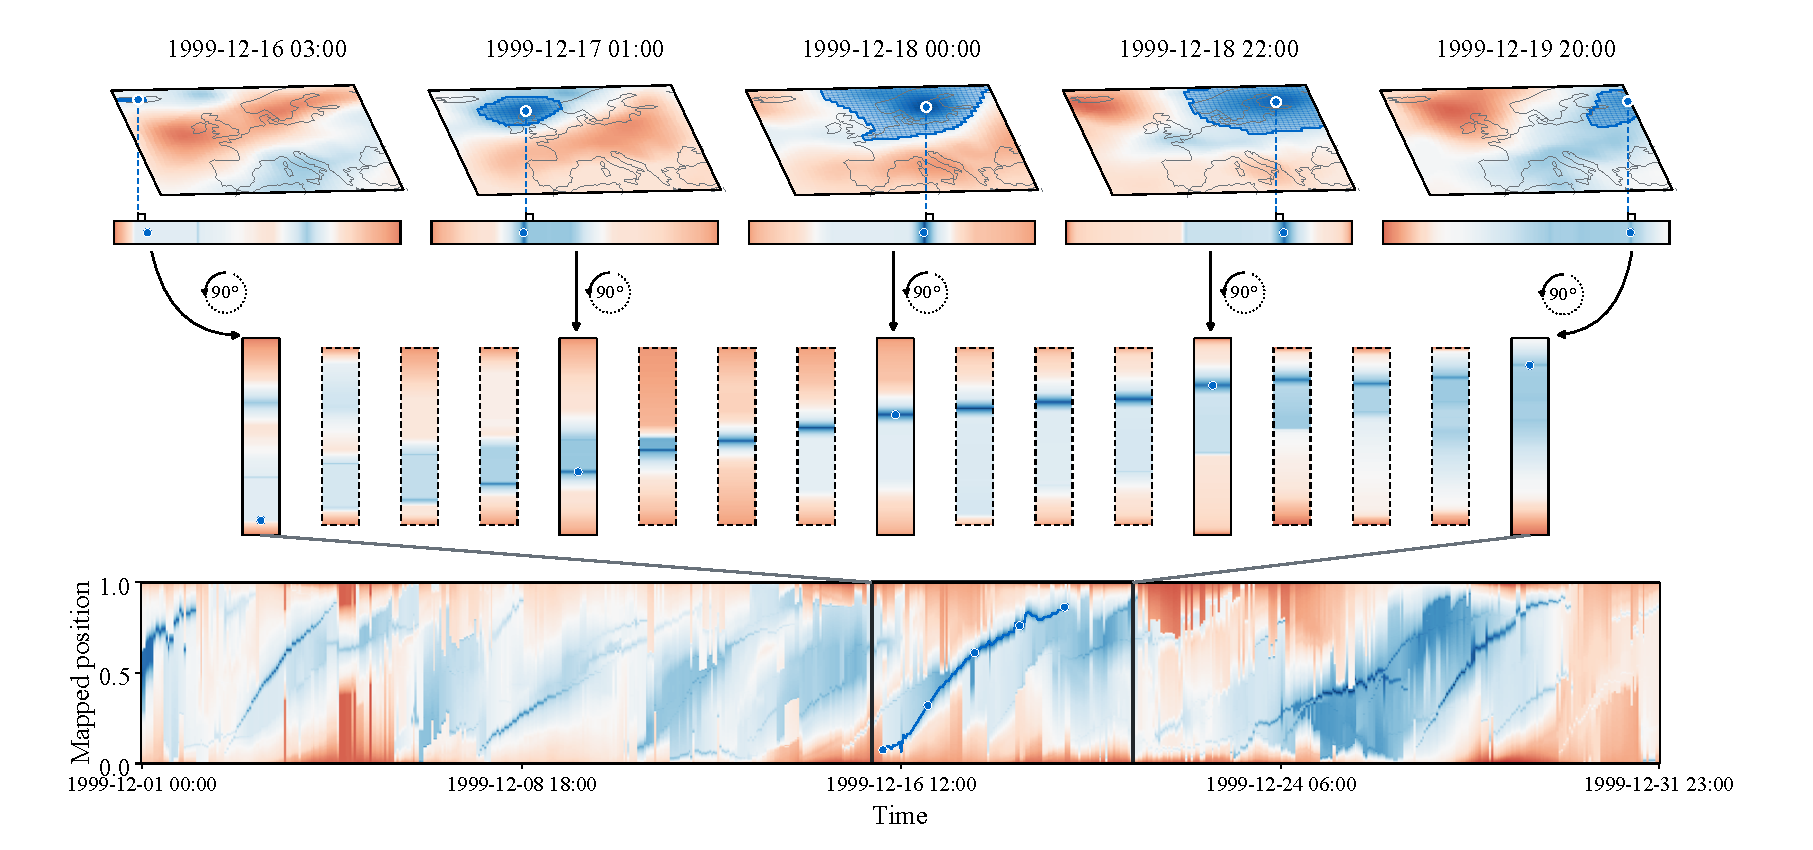
\includegraphics[width=\linewidth]{../figures/anchor_storms_overview.pdf}
\par
\refstepcounter{figure}\label{fig:storms_overview}
{\captionfonts\raggedright\noindent\figurename~\thefigure: Qualitative Storms archive ($\varepsilon=5\%$; preprocessing differs from Table~\ref{tab:quantitative-final}). Spatial snapshots and profiles identify one matched extremum; blue outlines show leaf-arc supports. Rotated profiles and dashed intermediate samples connect to its trajectory in the full 744-frame map.\par}

}
\linespread{0.90}
\setlength{\textfloatsep}{7pt}
\setlength{\floatsep}{6pt}
\setlength{\dbltextfloatsep}{7pt}
\begin{document}
\firstsection{Introduction}
\maketitle
\raggedbottom
\setlength{\emergencystretch}{1.5em}
2D and 3D time-varying scalar fields describe evolving phenomena such as pressure systems, combustion structures, and flow features. Their analysis requires understanding where features occur, how they move along a relevant spatial direction, and how their hierarchical relationships change throughout a sequence. Extrema and component merges describe this evolving scalar structure, while spatial coordinates connect it to the physical domain. A temporal overview should bring these aspects together. Figure~\ref{fig:storms_overview} illustrates how spatial supports and reference positions connect to scalar profiles and the resulting temporal map.

Animation preserves the spatial view at each instant, but comparison between distant times requires navigation and memory. Small multiples expose observations simultaneously at the cost of screen space. Static temporal summaries allocate one display axis to time and compress the spatial domain into the remaining axis~\cite{Tversky:2002:Animation,Robertson:2008:Animation,Bach:2017:STC}. Spatial linearization makes long sequences accessible in one image; the meaning of its 1D coordinate determines which spatial questions the overview can support.

Merge tree maps organize this compression around scalar features and their hierarchy. Temporal Merge Tree Maps (TMTM) linearize augmented merge trees into scalar profiles aligned across time~\cite{Koepp:2023:TMTM}. Minima and intervening barriers encode extrema and merge levels, exposing scalar structure and its temporal evolution. Spatiotemporal Merge Tree Maps (ST-MTM) incorporate relative spatial distances and temporal position constraints into a geometry-aware layout~\cite{STMTM:2026}. These methods provide the foundation for compact overviews of temporal scalar topology.

A display coordinate chosen for hierarchy, relative distance, or temporal alignment need not correspond to a fixed physical direction. Its position cannot then be read directly as longitude or distance along a flow axis, and its changes need not represent motion along that direction. Relative geometry supplies spatial relationships but leaves the absolute coordinate origin undetermined. The remaining question is how to give the temporal map a consistent spatial reference while retaining its hierarchical information.

The central question is whether displacement from a spatial reference is required by the hierarchy or introduced by a particular layout. Interleaved reference positions can conflict with the contiguous subtree blocks required by exact topology, but this does not imply that a merge tree map must abandon a spatial axis. A method-independent lower bound is needed to distinguish these cases. 

We derive three certified position bounds. The first gives the exact minimum reference-order error for a topology-preserving point layout and is attained by recursive midpoint ordering. The second includes finite feature widths, gaps and canvas boundaries. The third identifies restrictions that survive a declared merge-level allowance. These bounds apply to every map satisfying their assumptions, including maps produced by other objectives. In the point model, error above the exact bound is avoidable through reordering; for finite widths, a certificate gap may reflect either a loose bound or a suboptimal search.

AnchorMTM, \emph{Spatially Anchored Merge Tree Maps}, constructs maps within this model. One spatial reference is fixed across the sequence, using a standard leading eigenvector of matched-extremum motion or an analyst-supplied physical direction. A heuristic order search, capped spatiotemporal anchor optimization and checked scalar-profile reconstruction use a common merge-error allowance. Exact and budgeted modes expose how much spatial displacement can be reduced by changing the displayed hierarchy. Planar and volumetric comparisons examine reference alignment, achieved topology error and the spatial relationships visible in the resulting maps.

Our contributions comprise theoretical bounds, a layout construction and an empirical evaluation:
\begin{itemize}
\setlength{\itemsep}{2pt}
\setlength{\parsep}{0pt}
\item \emph{Certified position bounds.} Three certified bounds quantify the restrictions imposed by exact topology, finite widths and a bounded topology allowance, independently of the layout algorithm.
\item \emph{Topology-budgeted layout construction.} A topology-budgeted construction combines a shared reference with leaf ordering, capped anchor placement and explicit checks of reconstructed merge levels.
\item \emph{Evaluation of the position--topology trade-off.} Planar and volumetric comparisons document reference alignment, relative spatial quality and topology validity, with map examples illustrating the meaning of the shared coordinate.
\end{itemize}

% Former Figure 2 temporarily removed; source retained in figures/source/ring_result_20261106.

\section{Related Work}\label{sec:related}
\subsection{Spatially Referenced Temporal Visualization}
Static temporal displays expose distant observations simultaneously, while animation retains the spatial view of each instant; their usefulness depends on the analytical task~\cite{Tversky:2002:Animation,Robertson:2008:Animation}. Generalized space--time cubes describe the transformations connecting such views~\cite{Bach:2017:STC}. In compressed temporal overviews, the spatial coordinate determines which location and motion relationships remain directly interpretable.

Hovm\"oller diagrams retain a selected physical coordinate and summarize the other dimensions~\cite{Hovmoller:1949}. Geographic orderings and space-filling curves instead traverse the domain~\cite{Guo:2006:SpatialOrder,Dafner:2000:CSFC}. Dynamic Volume Lines and data-driven curves extend spatial traversal to volumetric comparison and scalar-aware ordering~\cite{Weissenboeck:2019:DVL,Zhou:2021:DSF}. A traversal can retain spatial neighborhoods, but its 1D coordinate is generally different from a fixed projection, and traversal adjacency alone does not enforce the merge hierarchy.

1D projections organize spatiotemporal phenomena~\cite{Franke:2021:1DP}, and MotionRugs expose collective behavior of moving entities~\cite{Buchmueller:2019:MR}. More generally, an embedding trades original-domain relationships against its display organization~\cite{Nonato:2019:MP}. Relative proximity does not determine an absolute coordinate. AnchorMTM assigns fixed projection targets to topological features and quantifies their displacement under hierarchical and interval constraints, combining spatial reference with a temporal topology overview.


\begin{figure}[t]
\centering
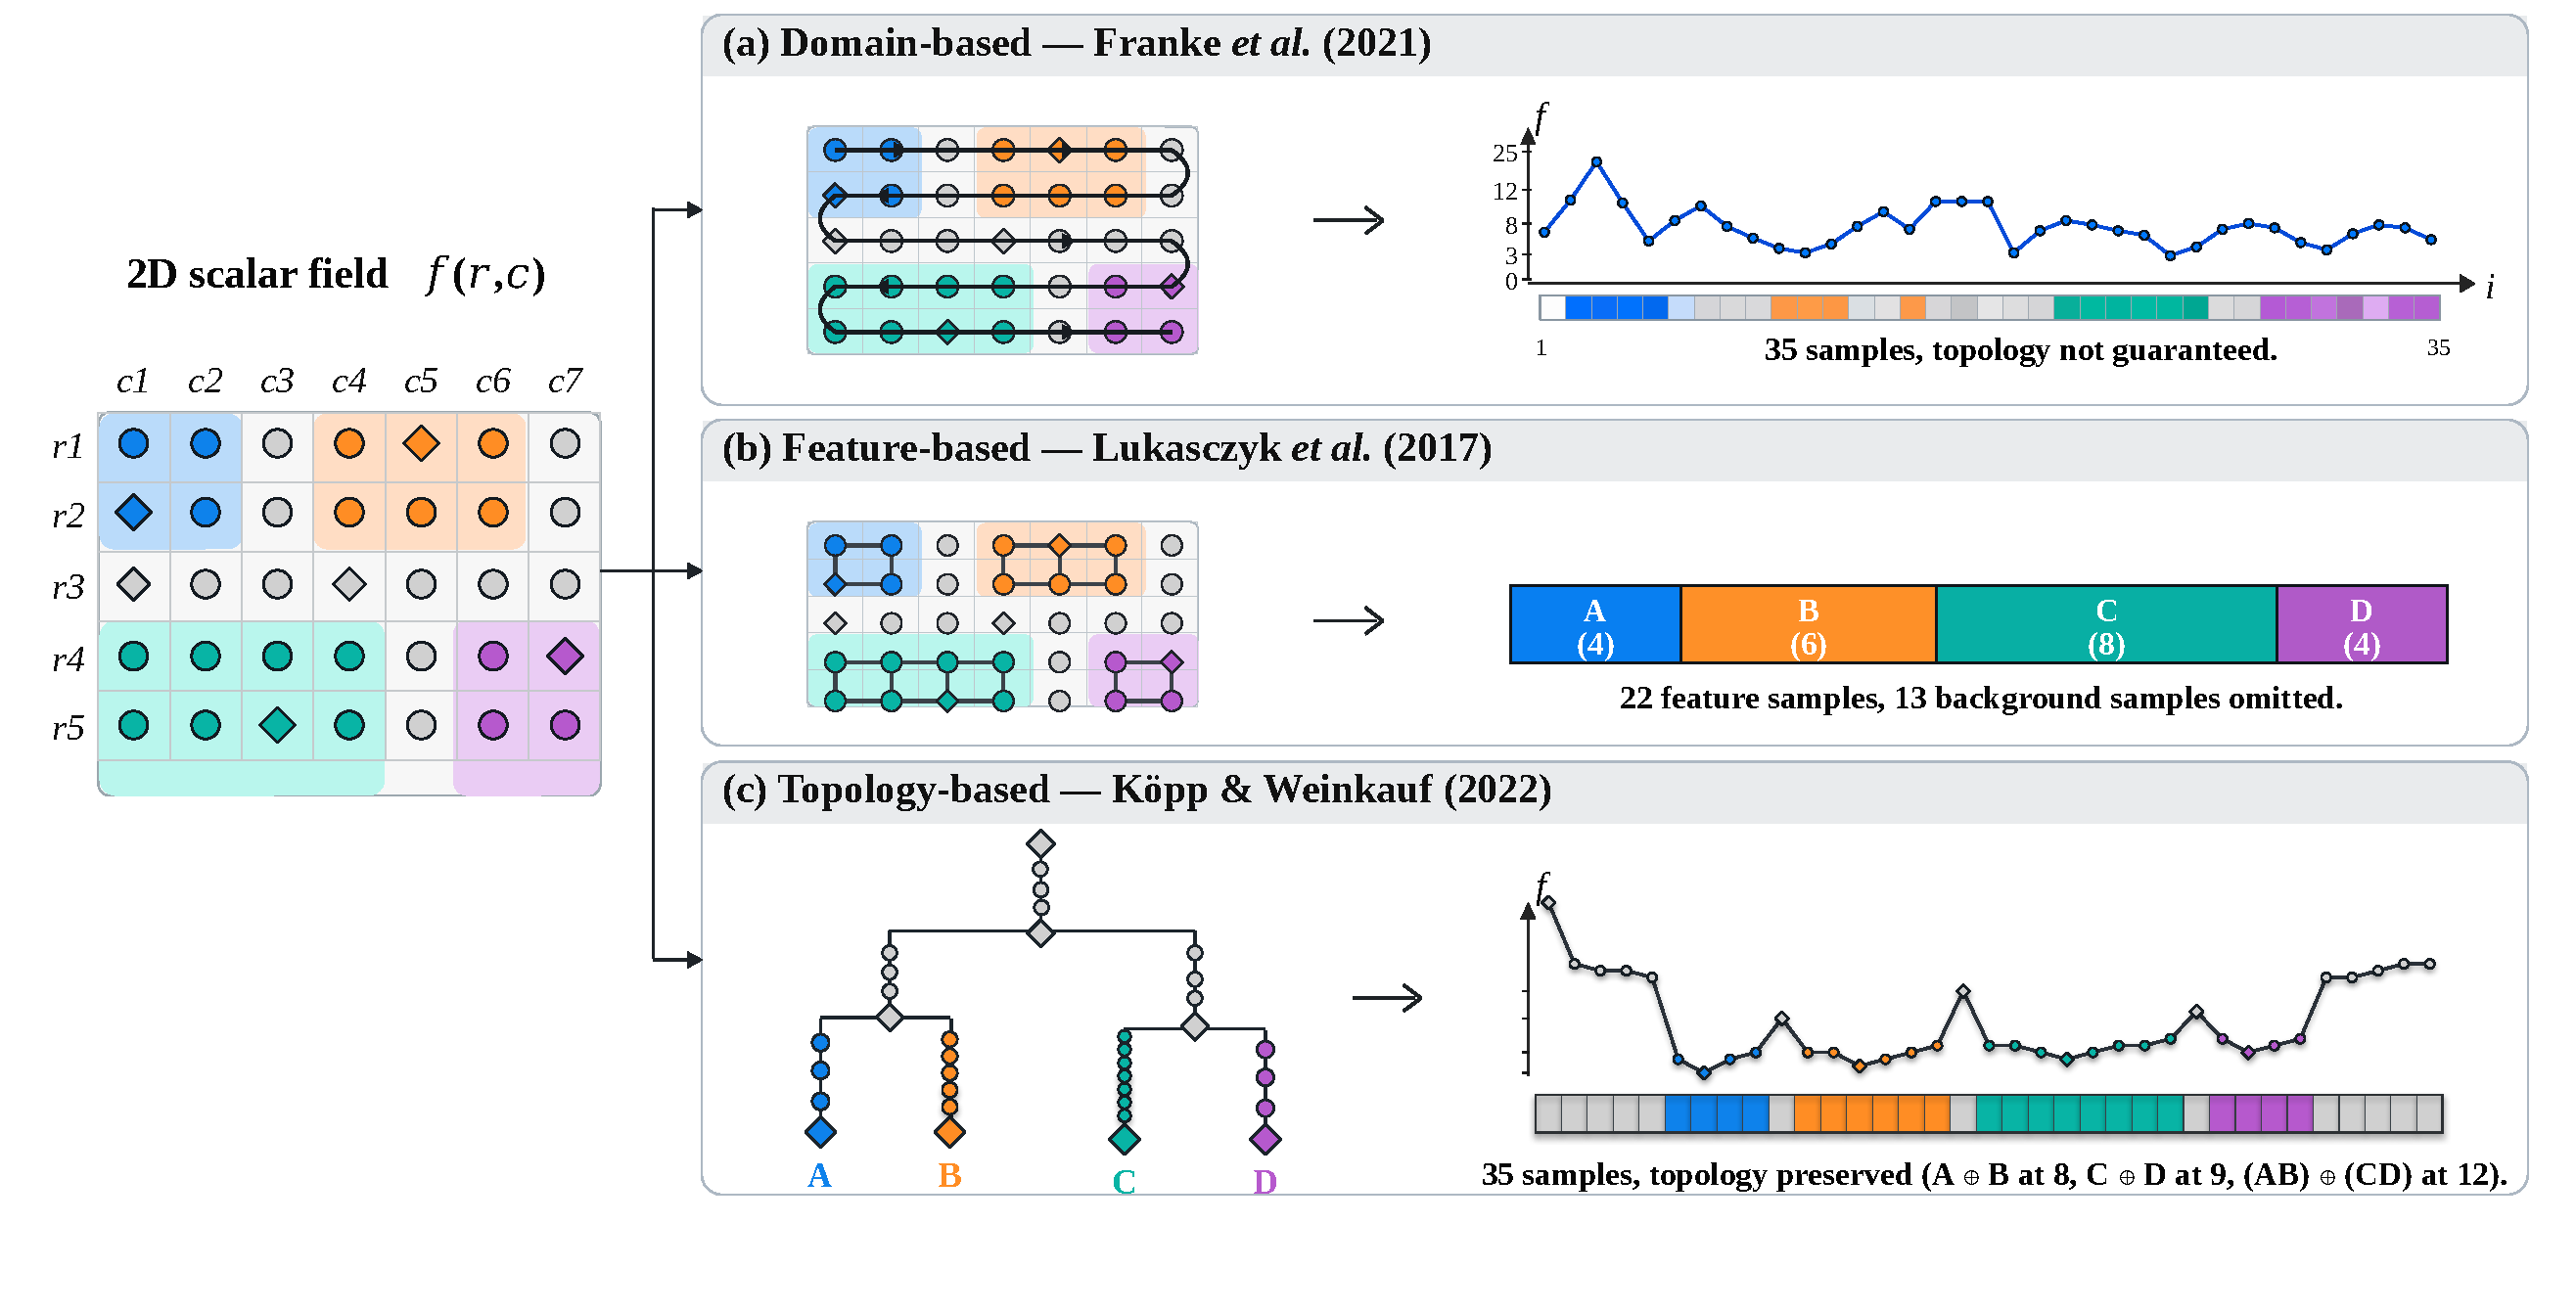
\includegraphics[width=\columnwidth]{../figures/anchor_related_work_mapping.pdf}
\caption{Schematic comparison of temporal mapping strategies on a shared 35-sample scalar field. (a) Domain-based traversal retains all samples without enforcing the merge hierarchy. (b) Feature-based summaries retain 22 selected feature samples and omit 13 background samples. (c) A topology-based profile retains all 35 samples while preserving the illustrated merge levels. Colored regions indicate the four example features; the drawings illustrate representation choices rather than measured benchmark outputs.}
\label{fig:related-work-mapping}
\end{figure}

\subsection{Topology-Based Temporal Maps and Geometry-Aware Layouts}
Figure~\ref{fig:related-work-mapping} contrasts domain-, feature-, and topology-based representations on the same schematic field. Topology-based visualization organizes scalar structures through connectivity~\cite{Heine:2016:Survey}. Landscapes and landscape profiles express hierarchies through terrain or 1D scalar representations~\cite{Weber:2007:TL,Oesterling:2013:TLP}, with geometry-preserving and temporally coherent extensions~\cite{Beketayev:2012:GPTL,Herick:2020:TCTL}. These representations connect scalar values and feature relationships in a compact view.

TMTM emphasizes intact topological features and temporal alignment in static merge-tree maps~\cite{Koepp:2023:TMTM}. ST-MTM incorporates relative spatial geometry and temporal position constraints~\cite{STMTM:2026}. These priorities give spatial relationships and coherence a role in the map, while leaving its display coordinate free to differ from a fixed physical direction. AnchorMTM estimates a shared direction from extremum motion, or accepts a physical direction, and couples that reference to topology-budgeted layout and certified position bounds. It reuses the established profile and scalar-filling foundation.

Hierarchy-constrained leaf ordering traditionally minimizes adjacent dissimilarity~\cite{BarJoseph:2001:OLO}; target-order reordering studies related tree-consistent permutations~\cite{Bulteau:2022:RT}. Separation-constrained layouts control geometric overlap and displacement~\cite{Dwyer:2006:IPSEP,Li:2019:SOI}. AnchorMTM couples these layout concerns to fixed spatial targets. Its exact-topology point-order bound has a closed form, whereas finite-width candidate ordering remains heuristic.

Merge-tree comparison depends on the descriptors and correspondences used~\cite{Yan:2021:Survey}. Labelled cophenetic/interleaving comparisons support fixed-identity merge-level accounting~\cite{Munch:2019:LINF,Gasparovic:2024:IID}, and ordered merge trees connect scalar curves to monotone interleaving distances~\cite{Beurskens:2025:OMT}. We use fixed labels to measure displayed merge error. The optimal-barrier subproblem relates to minimax ultrametric fitting~\cite{Farach:1995:RM}, with the additional restriction that one linear order induces every displayed merge.

\begin{figure*}[t]
\centering
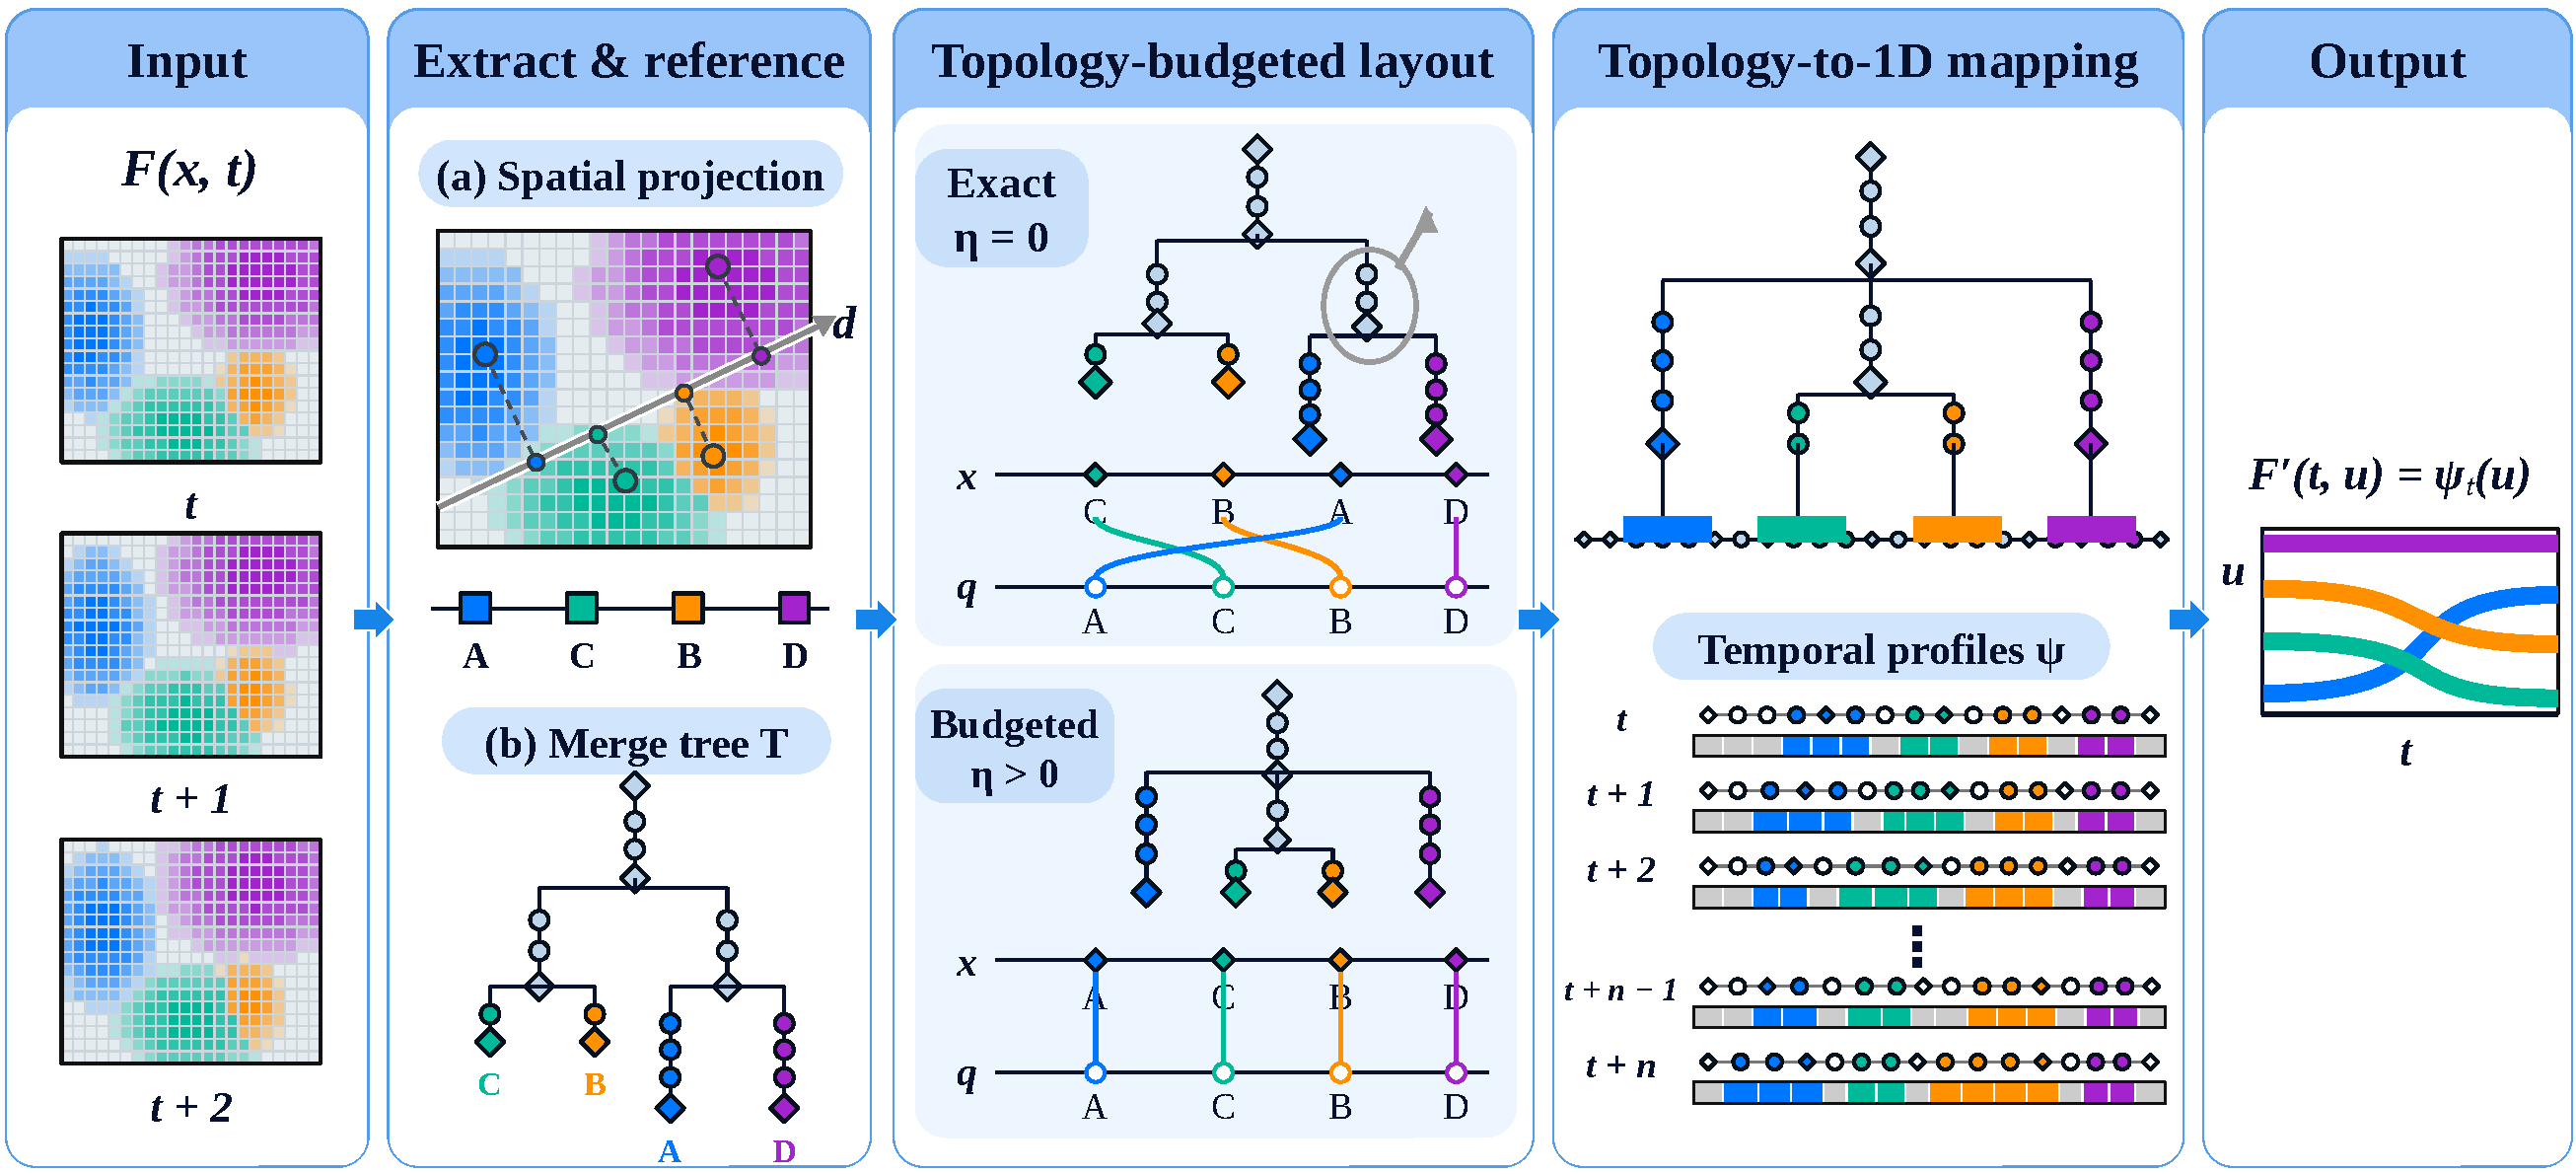
\includegraphics[width=\textwidth]{../figures/anchor_framework.pdf}
\caption{AnchorMTM construction. (1) Extract augmented merge trees and match leaf supports, then estimate one fixed spatial reference from matched extremum motion. (2) Refine candidate leaf orders, admit those satisfying the merge-error allowance, and select by fixed-order displacement and NROE. (3) Optimize anchors within nonoverlapping intervals under a displacement cap, using valid matched history. (4) Reconstruct scalar profiles with barrier correction and assemble the temporal map. Diagrams are schematic; the map is an existing qualitative Storms output at $\varepsilon=10\%$. }
\label{fig:framework}
\end{figure*}

\section{Merge-Tree Map Preliminaries}\label{sec:background}
\subsection{Augmented Merge Trees and Feature Supports}
For a sampled 2D or 3D field $f_t:D\to\mathbb{R}$, the merge tree $T_t$ records sublevel-set connectivity: minima create components and saddles join them as the threshold increases. Negating the field gives the split-tree convention. Critical points are supernodes connected by superarcs; augmentation associates regular vertices with these arcs~\cite{Koepp:2023:TMTM,STMTM:2026,Tierny:2018:TTK}. Extraction and simplification precede layout.

A leaf represents an extremum at spatial location $p_i^t$. Its feature support $S_i^t$ consists of that extremum and the regular samples on its incident leaf arc, excluding the parent critical sample. It is not the full component or the complete subtree above that arc. For cross-frame overlap, these supports are sets of stable spatial sample IDs: the same ID must denote the same spatial sample across frames. Fixed-grid inputs preserve this identity through consistent sample indexing. Internal arcs retain further regular samples for scalar filling. Write $\mathcal{D}_t(v)$ for the descendant leaf labels of a node $v$, and $h_t(v)$ for its scalar level. The lowest common ancestor determines the merge-height matrix:
\begin{equation}\label{eq:merge}
 V_{ij}^t=h_t(\lca(i,j)),\quad i\ne j;\qquad
 V_{ii}^t=f_t(p_i^t).
\end{equation}
Equal-level merge events form one multifurcation; arbitrary binary refinements do not add strict constraints. All subsequent guarantees refer to the supplied, possibly simplified tree.

\subsection{One-Dimensional Merge-Tree Profiles}
A 1D merge-tree profile represents extrema at anchors in a selected leaf order. Regular vertices on leaf arcs supply scalar context within leaf intervals; internal arcs and paths to the LCA supply the intervening gaps~\cite{Koepp:2023:TMTM,STMTM:2026}. In join convention, extrema become profile minima, and the largest profile value between two anchors gives their displayed merge level. Exact preservation requires each strict subtree to occupy a contiguous leaf block. Arranging these profiles along time yields a static temporal map. Figure~\ref{fig:node-mapping} illustrates sample identities across a tree and its 1D representation. This profile model provides the basis for the spatial anchoring formulation below.

\begin{figure}[t]
\centering
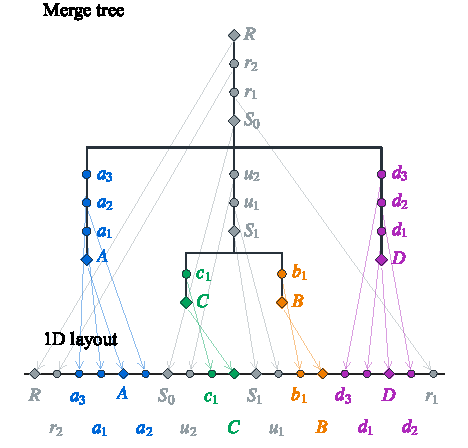
\includegraphics[width=\columnwidth]{../figures/anchor_node_mapping.pdf}
\caption{Renderer-checked filling example for one augmented join tree. First place leaf anchors $A,C,B,D$ and fill their colored leaf-arc intervals by alternating regular samples around each anchor. Then fill adjacent intervals using LCA barriers and internal-arc paths, and fill both outer borders along root paths. Gray internal-arc samples may be reused; the root critical node is not forced into a border sample. The 23 displayed values preserve all six pairwise leaf merge levels in this example. Positions illustrate filling, not an optimized experimental layout.}
\label{fig:node-mapping}
\end{figure}


\section{Spatial Anchoring: Formulation, Bounds and Construction}\label{sec:method}
Figure~\ref{fig:framework} summarizes the construction. We first fix the reference and define admissible maps, then derive bounds that apply to any such map, and finally describe how AnchorMTM searches and places a layout. This order separates what the constraints require from what the algorithm chooses. Analysis uses join convention; split-tree scalar signs are restored after reconstruction.

\subsection{Shared Spatial Reference and Layout Model}\label{sec:reference-model}
\paragraph{Cross-frame Leaf Correspondence.}
We track merge-tree leaf extrema $p_i^t$ using their leaf-arc supports $S_i^t$. On a shared fixed grid, overlap-based preprocessing~\cite{STMTM:2026} counts common spatial samples:
\begin{equation}\label{eq:overlap}
 O_{ij}^t=|S_i^t\cap S_j^{t+1}|.
\end{equation}
Hungarian assignment maximizes total intersection count over one-to-one pairs, discarding zero-overlap pairs. Figure~\ref{fig:leaf_correspondence} illustrates the resulting identity states.

\emph{Continuation} inherits a Track ID; \emph{birth/death} starts an unmatched current identity or ends an unmatched previous track. For \emph{non-bijective correspondence}, including potential one-to-many, many-to-one and ambiguous relations, only the assigned one-to-one links are retained. For a current leaf $i$, $\mu_t(i)$ denotes its valid predecessor. The layout receives precomputed tracks aligned to leaf rows; upstream support and confidence conventions are detailed in Supplementary Material.

\begin{figure}[tbp]
\centering
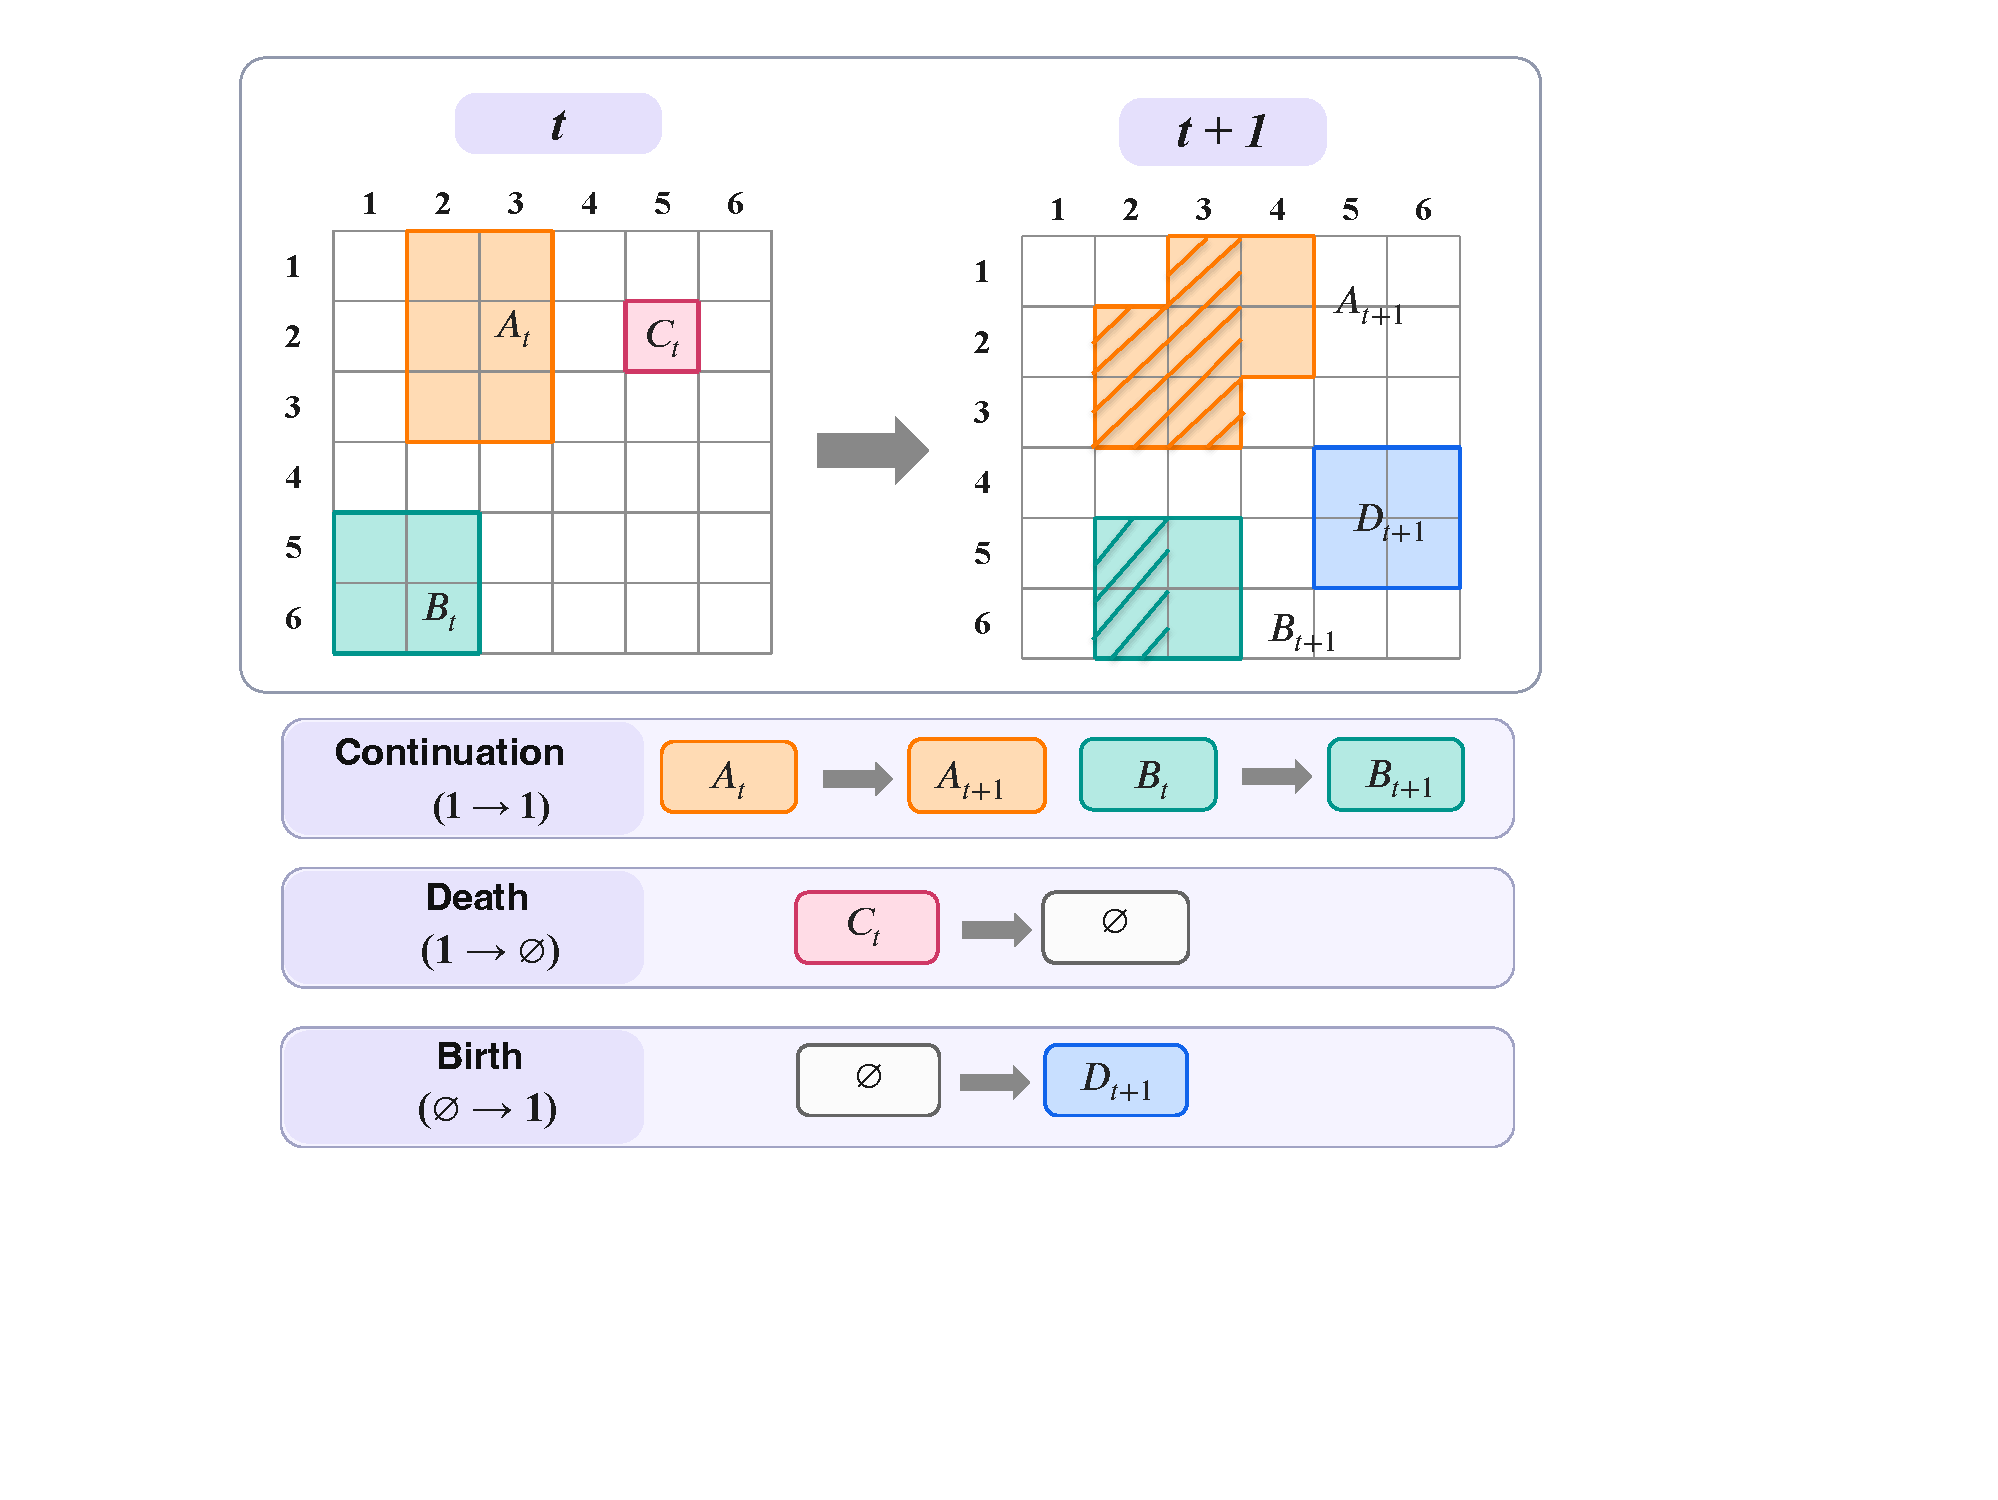
\includegraphics[width=\linewidth]{../figures/anchor_leaf_correspondence.pdf}
\caption{Overlap-based leaf correspondence on a shared grid. Colored regions represent leaf-arc supports; hatching marks samples shared with the previous frame. Maximum-overlap one-to-one assignment continues $A$ and $B$, leaves $C_t$ unmatched, and assigns a new identity to $D_{t+1}$. Birth and death denote matching states, not identified physical events.}
\label{fig:leaf_correspondence}
\end{figure}

These correspondences, computed before any topology-budget sweep, provide the motion samples for Spatial Anchoring, which distinguishes a reference target $q_i^t$ from the display anchor $x_i^t$. Only valid consecutive-frame matches contribute displacements; failed matches or interrupted tracks contribute no sample for that step. By default, one unit direction $a^*\in\mathbb{R}^d$, $d\in\{2,3\}$, is estimated offline from all matched consecutive-frame extremum displacements:
\begin{equation}\label{eq:autodirection}
\begin{aligned}
 \Delta p_i^t&=p_i^t-p_{\mu_t(i)}^{t-1},\\
 S&=\sum_{t,i\;\mathrm{matched}}\Delta p_i^t(\Delta p_i^t)^\top,\\
 a^*&\in\arg\max_{\|a\|=1}a^\top Sa.
\end{aligned}
\end{equation}
The leading eigenvector maximizes squared projected motion. The same calculation serves 2D and 3D; it is performed once for the whole sequence. Its sign makes total signed projected motion nonnegative; for near-zero signed motion, the largest-magnitude component is made positive. With negligible motion energy, the longest domain axis is used (first axis on a tie). Repeated leading eigenvalues leave the maximizing direction nonunique; the reported eigengap indicates this ambiguity. A supplied physical direction may replace $a^*$ without changing the layout. Overlap matching may miss fast-moving features or those with changing or weakly overlapping supports, affecting the displacement sample and hence the estimated direction.


For the selected direction, the minimum and span of the projected domain bounding-box corners define a common origin $o$ and extent $L>0$. The reference is
\begin{equation}\label{eq:reference}
 q_i^t=\langle a^*,p_i^t\rangle-o\in[0,L].
\end{equation}
Direction, origin and scale remain fixed across frames and all budgets for the same prepared sequence. Distinct extrema can share projected coordinates while retaining separate identities. Anchoring minimizes constrained deviation rather than requiring $x_i^t=q_i^t$.

Relative geometry uses distances $d_{ij}^t$ between leaf-support centroids. These differ from extremum references because a changing support can move its centroid while the extremum stays fixed. Widths $W_i^t=s\,m_i^t$ convert positive support measures with a fixed scale $s$, without per-frame normalization.

For example, consider four minima. The projected order $A,C,D,B$ separates $A$ and $B$ by the $C,D$ subtree, violating the required contiguity of $\{A,B\}$; exact topology therefore cannot realize all four targets without displacement.

With correspondence and the reference fixed, a frame comprises a leaf order, extremum anchors, and a scalar profile:
\begin{equation}\label{eq:mapframe}
 M_t=(\pi_t,x_t,\psi_t),\qquad\psi_t:[0,L]\to\mathbb{R}.
\end{equation}
We seek reference-aligned positions and motion while approximating relative geometry and controlling displayed topology. The interval-layout set $\mathcal{L}(\pi)$ requires intervals of widths $W_i$ centered at $z_i$ to lie inside the canvas, remain disjoint with gap at least $g\ge0$, and contain anchors satisfying $|x_i-z_i|\le\rho W_i/2$, $0\le\rho\le1$. Infeasible total widths and gaps are reported rather than rescaled.

Actual displacement is $|x_i-q_i|$, normalized by $L$ when reported. To distinguish order conflict from finite-width placement, define
\begin{equation}\label{eq:nroe}
 \nroe(\pi)=\frac{1}{2L}\max_{j\le k}
                      [q_{\pi(j)}-q_{\pi(k)}]^+.
\end{equation}
This is the smallest worst displacement of a nondecreasing point placement, divided by $L$; it ignores widths. For finite intervals, the exact fixed-order cost is
\begin{equation}\label{eq:tau}
 \tau(\pi)=\min_{(x,z)\in\mathcal{L}(\pi)}\|x-q\|_\infty.
\end{equation}
The minimum is attained whenever the layout set is nonempty. It is evaluated exactly from the fixed-order packing constraints, equivalently through a minimax linear program.

For distinct labels, let $V_{ij}^{\psi}$ be the maximum profile value between their anchors, with $V_{ii}^{\psi}=\psi(x_i)$. We require
\begin{equation}\label{eq:dtop}
\begin{aligned}
 \dtop(\psi_t,T_t)&=\max_{i,j}|V_{ij}^{\psi_t}-V_{ij}^t|\le\eta,\\
 \eta&=(\varepsilon_0+\varepsilon)\Delta_F.
\end{aligned}
\end{equation}
Here $\Delta_F>0$ is the sequence-wide scalar range, $\varepsilon_0$ is a fixed numerical allowance, and $\varepsilon\ge0$ is the sole primary user control. The implementation defaults to $\varepsilon_0=10^{-7}$. NMLE reports the achieved normalized error $\dtop/\Delta_F$. Exact topology means zero labelled error on the declared tree.

All remaining settings belong to a fixed configuration $\Theta_0$: position slack $\beta_0$, the four objective weights, width scale, gap, anchor slack and output resolution. For a prepared sequence, the default interface is $M_t^\varepsilon=\operatorname{AnchorMTM}(T_t,q_t,W_t,V_t,\mu_t;\varepsilon,\Theta_0)$. Advanced settings may be supplied once, but only $\varepsilon$ varies in a budget sweep. Supplementary Material specifies the fixed scale rules and implementation tolerances.

For canonical cophenetic merge-tree representations whose fixed labels cover every leaf and whose induced matrices include the diagonal, $\dtop$ equals the unnormalized labelled interleaving distance~\cite{Munch:2019:LINF,Gasparovic:2024:IID}. Under these conditions, $d_B\le d_I\le\dtop$~\cite{Morozov:2013:IDMT}. 


\subsection{Certified Position--Topology Bounds}\label{sec:bounds}
How much must any admissible map deviate from its reference? The following bounds isolate what topology and finite widths make unavoidable: the first answers how much a tree-compatible point order must deviate, the second adds interval packing, and the third asks which restrictions survive a merge-error allowance. The resulting certificates apply independently of the layout algorithm. Full proofs and computational definitions accompany the paper in Supplementary Material. We suppress $t$ within a frame, use $[v]^+=\max(v,0)$, and take empty maxima as zero.

\subsubsection{Exact-Topology Reference-Order Bound}
For a reduced tree with strictly increasing proper-ancestor levels, exact topology makes every subtree contiguous. Let $[m_X,M_X]$ be the reference hull of the leaves in subtree $X$.
\begin{theorem}[Exact-Topology Position Bound]\label{thm:order}
Every zero-error profile has $\nroe(\pi)\ge\nu^*(T,q)$, where
\begin{equation}\label{eq:nu}
 \nu^*(T,q)=\frac{1}{2L}\max_v\max_{\substack{X,Y\in\mathrm{ch}(v)\\X\ne Y}}
 [\min(M_X-m_Y,M_Y-m_X)]^+.
\end{equation}
Recursive child ordering by reference-hull midpoint attains this point-model order bound in $O(n\log n)$ time.
\end{theorem}
\begin{proof}[Proof sketch]
Sibling blocks must choose one orientation. Their two possible inversion costs are $[M_X-m_Y]^+/2$ and $[M_Y-m_X]^+/2$. Midpoint order chooses the smaller; every inverted leaf pair is separated by sibling blocks at its LCA.
\end{proof}
This result isolates the ordering restriction imposed by the tree and references. Midpoint ordering attains the point-order optimum; finite intervals introduce additional constraints, considered next.

\subsubsection{Width-Aware Position Bound}
Finite widths, minimum gaps, anchor slack and canvas capacity add packing costs to the point-order obstruction. For a nonempty leaf set $S$, let $H_i=\rho W_i/2$, $\ell_i=q_i-W_i/2-H_i$, $h_i=q_i+W_i/2+H_i$, and $s_i=W_i+g$. Define two packing summaries:
\begin{equation}\label{eq:packing}
\begin{aligned}
 A(S)&=\max_{a\in S}\left(\ell_a+\sum_{\substack{i\in S\\\ell_i\ge\ell_a}}s_i\right),\\
 B(S)&=\max_{b\in S}\left(\sum_{\substack{i\in S\\h_i\le h_b}}s_i-h_b\right).
\end{aligned}
\end{equation}
The first uses upper reference-endpoint sets and the second lower sets; sorting and cumulative sums evaluate them. For disjoint leaf sets $X,Y$ and the full leaf set $\mathcal{F}$, write
\begin{equation}\label{eq:packingcost}
\begin{aligned}
 \omega(X,Y)&=\tfrac12\min\{A(X)+B(Y),A(Y)+B(X)\}-\tfrac g2,\\
 E_\partial&=\max\{0,B(\mathcal{F})-g,A(\mathcal{F})-g-L\}.
\end{aligned}
\end{equation}
Here $\omega$ takes the cheaper block orientation and $E_\partial$ accounts for both canvas ends. Let $\mathcal{P}_0$ contain every pair of distinct sibling descendant-leaf sets. The certificate is
\begin{equation}\label{eq:bwdef}
 \mathcal{B}_w(T,q,W)=\max\{E_\partial,\max_{(X,Y)\in\mathcal{P}_0}\omega(X,Y)\}.
\end{equation}
The dependence on $g$, $\rho$ and $L$ is through Eqs.~\ref{eq:packing}--\ref{eq:packingcost}; it is suppressed in the certificate's arguments.
\begin{theorem}[Width-Aware Position Bound]\label{thm:width}
For any feasible exact-topology interval layout,
\begin{equation}\label{eq:widthbound}
 \|x-q\|_\infty\ge\tau(\pi)\ge\mathcal{B}_w(T,q,W).
\end{equation}
With zero widths and gaps, $\mathcal{B}_w=L\nu^*(T,q)$.
\end{theorem}
\begin{proof}[Proof sketch]
The first and last anchors of selected leaves must enclose their intervals and intervening gaps, up to the allowed anchor slack. Upper and lower sets in Eq.~\ref{eq:packing} maximize the resulting shortfall against reference separation. Exact topology requires one orientation of every sibling pair; the canvas ends give the two one-sided costs.
\end{proof}
Thus $\mathcal{B}_w$ bounds all exact-topology legal interval orders and need not be attained; $\tau(\pi)$ is the attained minimum for a specified order. These quantities have coordinate units, whereas NROE and $\nu^*$ are normalized by $L$.

\begin{table}[t]
\centering
\caption{Balanced-mode parameters and runtime (seconds) on Apple M4; one measured run per dataset.}
\label{tab:anchor-parameters-final}
\footnotesize
\setlength{\tabcolsep}{3pt}
\resizebox{\columnwidth}{!}{%
\begin{tabular}{lrrrrr}
\toprule
Dataset & $\varepsilon$ & $L$ & $s_w$ & $t_{opt}$ & $t_{total}$ \\
\midrule
Gaussian & 1\% & 4096 & 0.00581 & 0.156 & 1.340 \\
\addlinespace[2pt]
Ring & 1\% & 196 & 0.00328 & 0.150 & 0.486 \\
\addlinespace[2pt]
Wildfires & 5\% & 4096 & 0.00053 & 3.324 & 4.424 \\
\addlinespace[2pt]
Storms & 10\% & 4096 & 0.01170 & 2.600 & 63.447 \\
\addlinespace[2pt]
\bottomrule
\end{tabular}
}
\vspace{3pt}
\begin{minipage}{\columnwidth}\footnotesize Weights $(4,1,0.5,0.1)$ and $\rho=0.5$ are fixed. $s_w$ is width per support measure; $L$ is raster length. Optimization covers ordering/placement; total includes the full pipeline.\end{minipage}
\end{table}

\begin{table*}[t]
\centering
\caption{Four-dataset quantitative comparison. TMTM and ST-MTM (Temporal mode) SNS/TW are reported values from ST-MTM Table~1; AnchorMTM values and all NPE values are locally measured. Bold/underline mark the best/second distinct displayed value within each dataset, including ties. This numerical comparison does not establish identical author inputs or evaluation coverage.}
\label{tab:quantitative-final}
\small
\setlength{\tabcolsep}{4pt}
\resizebox{\textwidth}{!}{%
\begin{tabular}{lrrrrrrlrrr}
\toprule
\multirow{2}{*}{Dataset} & \multicolumn{3}{c}{TMTM} & \multicolumn{3}{c}{ST-MTM} & \multicolumn{4}{c}{AnchorMTM (our method)} \\
\cmidrule(lr){2-4}\cmidrule(lr){5-7}\cmidrule(lr){8-11}
 & SNS$\downarrow$ & TW$\uparrow$ & NPE$\downarrow$ & SNS$\downarrow$ & TW$\uparrow$ & NPE$\downarrow$ & Mode & SNS$\downarrow$ & TW$\uparrow$ & NPE$\downarrow$ \\
\midrule
\multirow{2}{*}{Gaussian} & \multirow{2}{*}{$0.2500$} & \multirow{2}{*}{$0.7700$} & \multirow{2}{*}{$\underline{0.1118}$} & \multirow{2}{*}{$\underline{0.0600}$} & \multirow{2}{*}{$\mathbf{1.0000}$} & \multirow{2}{*}{$0.1154$} & Exact & $\mathbf{0.0353}$ & $\underline{0.9323}$ & $\mathbf{0.0089}$ \\
 &  &  &  &  &  &  & Balanced & $\mathbf{0.0353}$ & $\underline{0.9323}$ & $\mathbf{0.0089}$ \\
\addlinespace[2pt]
\multirow{2}{*}{Ring} & \multirow{2}{*}{$0.2800$} & \multirow{2}{*}{$0.6800$} & \multirow{2}{*}{$0.1756$} & \multirow{2}{*}{$0.2100$} & \multirow{2}{*}{$\mathbf{0.8800}$} & \multirow{2}{*}{$0.2463$} & Exact & $\underline{0.1485}$ & $\underline{0.8571}$ & $\underline{0.0471}$ \\
 &  &  &  &  &  &  & Balanced & $\mathbf{0.1334}$ & $\underline{0.8571}$ & $\mathbf{0.0395}$ \\
\addlinespace[2pt]
\multirow{2}{*}{Wildfires} & \multirow{2}{*}{$0.4400$} & \multirow{2}{*}{$0.8800$} & \multirow{2}{*}{$0.2280$} & \multirow{2}{*}{$0.2400$} & \multirow{2}{*}{$\underline{0.9100}$} & \multirow{2}{*}{$0.3180$} & Exact & $\mathbf{0.0426}$ & $\mathbf{0.9136}$ & $\underline{0.0131}$ \\
 &  &  &  &  &  &  & Balanced & $\underline{0.0447}$ & $0.8989$ & $\mathbf{0.0116}$ \\
\addlinespace[2pt]
\multirow{2}{*}{Storms} & \multirow{2}{*}{$0.3400$} & \multirow{2}{*}{$0.7100$} & \multirow{2}{*}{$0.5753$} & \multirow{2}{*}{$0.2100$} & \multirow{2}{*}{$\mathbf{0.9400}$} & \multirow{2}{*}{$0.4579$} & Exact & $\underline{0.0790}$ & $0.8463$ & $\underline{0.0399}$ \\
 &  &  &  &  &  &  & Balanced & $\mathbf{0.0743}$ & $\underline{0.8766}$ & $\mathbf{0.0140}$ \\
\addlinespace[2pt]
\bottomrule
\end{tabular}
}
\vspace{3pt}
\begin{minipage}{\textwidth}\footnotesize Mode applies to AnchorMTM; baseline entries are shared by both rows. TW uses $k=1,3,5,3$ for Gaussian, Ring, Wildfires and Storms. AnchorMTM TW coverage is respectively 64/64, 1/40, 4/32 and 11/744 in both modes; author coverage is unspecified. Ineligible frames are omitted. Published TW values have only two decimal places, so apparent small differences are not evidence of superiority.\end{minipage}
\end{table*}

\subsubsection{Bounded-Topology Position Bound}
A merge-level allowance can release some contiguous blocks, but still limits interleaving. If leaf $k$ lies between descendants $i,j$ of node $u$, interval containment gives $V_{ik}^{\psi}\le V_{ij}^{\psi}$, hence $V_{ik}\le h(u)+2\eta$. Define $A_\eta(u)$ as the highest ancestor, including $u$, with $h(A_\eta(u))-h(u)\le2\eta$. This uses the accumulated ancestor-height difference in scalar units, on the reduced equal-level tree with the fixed labels of Eq.~\ref{eq:dtop}.

Let $\mathcal{P}_\eta$ consist of two types of leaf-set pairs: $(\mathcal{D}(u),\{k\})$ for every internal node $u$ and leaf $k\notin\mathcal{D}(A_\eta(u))$; and $(\mathcal{D}(u),\mathcal{D}(w))$ for internal nodes $u,w$ satisfying
\begin{equation}\label{eq:separatedpairs}
\begin{aligned}
 \mathcal{D}(w)\cap\mathcal{D}(A_\eta(u))&=\varnothing,\\
 \mathcal{D}(u)\cap\mathcal{D}(A_\eta(w))&=\varnothing.
\end{aligned}
\end{equation}
For any nonempty leaf set $X$, use its reference hull $[m_X,M_X]$ and define $\kappa(X,Y)=[\min(M_X-m_Y,M_Y-m_X)]^+/(2L)$. The two certificates are
\begin{equation}\label{eq:chaindef}
\begin{aligned}
 C_\eta(T,q)&=\max_{(X,Y)\in\mathcal{P}_\eta}\kappa(X,Y),\\
 C_{w,\eta}(T,q,W)&=\max\{E_\partial,\max_{(X,Y)\in\mathcal{P}_\eta}\omega(X,Y)\}.
\end{aligned}
\end{equation}
\begin{theorem}[Bounded-Topology Position Bound]\label{thm:chain}
In a profile with $\dtop\le\eta$, no leaf outside $\mathcal{D}(A_\eta(u))$ can lie between two leaves of $u$. Every pair in $\mathcal{P}_\eta$ lies wholly in one block orientation or the other. Consequently,
\begin{equation}\label{eq:chainbounds}
 \nroe(\pi)\ge C_\eta(T,q),\qquad
 \tau(\pi)\ge C_{w,\eta}(T,q,W),
\end{equation}
with the second inequality applying to the interval model.
\end{theorem}
The separation principle excludes interleaving for each eligible pair; the two possible orientations then yield $\kappa$ and $\omega$. Thus $C_\eta$ bounds normalized reference-order error, while $C_{w,\eta}$ includes finite-width and boundary costs in coordinate units. Flattening every parent gap at most $2\eta$ and applying Theorems~\ref{thm:order} and~\ref{thm:width} to the remaining tree gives another valid certificate. Neither construction dominates: accumulated gaps can strengthen the chain certificate, whereas flattening also separates pairs of single leaves omitted by $\mathcal{P}_\eta$. The larger of the two valid bounds may be used.

\paragraph{Interpretation.}
The three bounds distinguish ordering conflicts, finite-width packing and restrictions that remain under a topology allowance. They explain why some reference displacement can persist even after optimization. In the point model, midpoint ordering attains the exact-topology bound; with finite widths, a gap above a lower bound need not be entirely avoidable because the bound itself may be loose. 

The allowance concerns the displayed hierarchy; the source field and feature identities stay fixed. These bounds are reported as benchmarks for unavoidable error; ranking and continuous acceptance use the exact fixed-order evaluations in Section~\ref{sec:construction}. 

\subsection{Topology-Budgeted Map Construction}\label{sec:construction}
With features and their reference fixed, construction chooses an order by the lexicographic objective
\begin{equation}\label{eq:orderobjective}
\begin{aligned}
 \pi_t^\varepsilon&\in\underset{\pi\in\mathcal{C}_t(\varepsilon)}{\arg\min}
                    \bigl(\tau_t(\pi),\nroe_t(\pi)\bigr),\\
 &\hspace{1em}\mathrm{s.t.}\quad\delta_t^*(\pi)\le\eta(\varepsilon).
\end{aligned}
\end{equation}
The finite candidate pool contains the original strict-topology order, midpoint initializations, and orders visited during width-aware refinement of threshold and selective flattenings. Every candidate is evaluated against the same source merge matrix. Selection minimizes $\tau$ first and NROE second. Algorithm~\ref{alg:construction} separates this discrete selection from fixed-order placement.

\begin{algorithm}[htbp]
\caption{Single-Control AnchorMTM}\label{alg:construction}
\KwData{2D/3D field sequence and grid; $\varepsilon\ge0$; fixed configuration $\Theta_0$.}
\KwResult{Temporal map $I^\varepsilon$, error records, or a failure report.}
Extract augmented trees, leaf supports and extrema; match supports and assign Track IDs\;
Estimate one direction and fixed references $q_t$; reuse this preprocessing across budgets\;
$\eta\leftarrow(\varepsilon_0+\varepsilon)\Delta_F$\;
\For{each time step $t$ in temporal order}{
 Report and stop if widths and gaps exceed the fixed canvas\;
 $\mathcal{C}_t\leftarrow\operatorname{GenerateAndRefine}(T_t,q_t,W_t,V_t,\eta)$; retain strict-topology candidates\;
 Evaluate $\tau(\pi)$, $\nroe(\pi)$ and $\delta^*(\pi)$ for candidates\;
 $\mathcal{F}_t\leftarrow\{\pi\in\mathcal{C}_t:\delta^*(\pi)\le\eta\}$\;
 \lIf{$\mathcal{F}_t=\varnothing$}{report no feasible candidate and stop}
 Select $\pi_t^\varepsilon$ from $\mathcal{F}_t$ by $(\tau,\nroe)$\;
 Compute optimal merge barriers for $\pi_t^\varepsilon$\;
 Solve the four-term QP only for $\pi_t^\varepsilon$, with cap $\tau(\pi_t^\varepsilon)+\beta_0$ and valid matched history\;
 Reconstruct the profile by leaf/LCA filling and barrier correction\;
 Record candidate counts, continuous and rendered errors, motion and failures; append profile to $I^\varepsilon$\;
}
\KwReturn{$I^\varepsilon$ and diagnostic records}\;
\end{algorithm}

\subsubsection{Topology-Budgeted Leaf Ordering}
\emph{Exact Mode} sets $\eta=0$ and requires zero labelled merge error on the supplied tree. \emph{Budgeted Mode} permits $\eta>0$. Setting only the additional budget $\varepsilon=0$ while retaining $\varepsilon_0>0$ gives a numerical allowance, not zero labelled error. Both modes share the same interval model and placement objective.

Candidate generation includes the exact tree, threshold flattenings, and a conflict-driven selective flattening. Midpoint orders initialize these structures. Width-aware block insertion refines the four best initial structures, together with the exact tree, while retaining the point-model budget order as a candidate. Moves improve the lexicographic score consisting of $\tau$ and a squared packing-residual term, and must pass $\delta^*(\pi)\le\eta$. Visited initial and trial orders are retained in the deduplicated pool, including the strict-tree initialization and retained point candidate. Final budget filtering and lexicographic selection use the exact fixed-order costs. 

Figure~\ref{fig:selective_relaxation} illustrates the additional ordering freedom created by a selective flattening. Removing the $A$--$B$ sibling constraint admits the order $A,C,D,B$ while retaining the $C$--$D$ subtree. This structural proposal still requires evaluation against the original merge matrix and the prescribed error budget.

The exact-tree structure remains a refinement seed, and its child-block moves preserve strict topology. Widths, gaps and canvas scale remain fixed throughout the search. Capacity failures, empty admitted sets and numerical solver errors are reported separately.

\subsubsection{Optimal Merge Barriers and Topological Feasibility}
For a fixed order, a pair's displayed merge is the largest intervening barrier. Set $C_k=\min_{i\le k<j}V_{\pi(i)\pi(j)}$ and $F_k=\max(V_{\pi(k)\pi(k)},V_{\pi(k+1)\pi(k+1)})$ for gap $k$.
\begin{proposition}[Optimal barriers]\label{prop:barriers}
With fixed extremum values in the continuous non-strict model, the smallest labelled merge error is
\begin{equation}\label{eq:delta}
\begin{split}
 \delta^*(\pi)=\max\bigg\{&0,\max_k(F_k-C_k),\\
 &\frac12\max_{i<j}\left(V_{\pi(i)\pi(j)}-
                         \max_{i\le k<j}C_k\right)\bigg\},
\end{split}
\end{equation}
and barriers $b_k=C_k+\delta^*(\pi)$ attain it.
\end{proposition}
Error $\delta$ requires $F_k\le b_k\le C_k+\delta$. Choosing the largest admissible barriers satisfies every pair's lower merge requirement exactly when $\delta\ge\delta^*$. Thus the order meets the merge-level allowance in this continuous model exactly when $\delta^*(\pi)\le\eta$. 

\subsubsection{Constrained Spatiotemporal Anchor Placement}
Once the order is fixed, the core terms are $E_R$, mean squared deviation from the fixed reference, and $E_M$, mean squared error in matched projected motion. The auxiliary term $E_G$ approximates support-centroid distances through ordered anchor separations; $E_C$ regularizes anchor offsets from interval centers. All four terms and their nonnegative weights are retained:
\begin{equation}\label{eq:qp}
\begin{aligned}
 \min_{x_t,z_t}\quad&\lambda_R E_R+\lambda_G E_G+\lambda_M E_M+\lambda_C E_C\\
 \mathrm{s.t.}\quad&(x_t,z_t)\in\mathcal{L}(\pi_t),\\
 &\|x_t-q_t\|_\infty\le\tau(\pi_t)+\beta_0.
\end{aligned}
\end{equation}
For each valid match, set $\Delta q_i^t=q_i^t-q_{\mu_t(i)}^{t-1}$ and use the previous display anchor plus this reference displacement as the temporal target:
\begin{equation}\label{eq:temporal_target}
 \hat x_i^t=x_{\mu_t(i)}^{t-1}+(q_i^t-q_{\mu_t(i)}^{t-1}).
\end{equation}
Thus $E_M$ follows projected motion while favoring continuity of $x-q$. First-frame, newly born and otherwise unmatched leaves have no previous-frame motion penalty. Each term is averaged over its features, ordered pairs or valid matches; the current automatic-reference adapter uses unit confidence for valid matches. 

Only $\varepsilon$ changes the topology allowance $\eta(\varepsilon)$. The fixed slack $\beta_0\ge0$ bounds additional position deviation after ordering. Because $\tau(\pi_t)$ is attained, the cap admits a feasible placement for the selected order. The convex QP balances the four objectives within this cap, processing frames in temporal order.

\subsubsection{Profile Reconstruction and Error Evaluation}
Reconstruction inherits the leaf-arc sampling and LCA-path filling of the merge tree map pipeline~\cite{Koepp:2023:TMTM,STMTM:2026}. Original extrema remain at their anchors; regular samples provide scalar context within intervals and gaps. Optimal-barrier correction then clips each inter-anchor interior to $b_k$ and raises an existing peak if necessary. This separate correction is required for relaxed orders; inherited LCA filling alone does not enforce the minimax barriers.

A common direction, origin, extent, and pixel conversion are used for all frames. The profiles form the final temporal map,
\begin{equation}\label{eq:map}
 I^\varepsilon(t,u)=\psi_t^\varepsilon(u),\qquad 0\le u\le L.
\end{equation}
Strict-extremum clearance and raster rounding can change the achieved error, so the reconstructed profile is evaluated after rendering. Records distinguish the requested allowance, position certificates, attained $\tau$, continuous $\delta^*$ and rendered merge error. Raster-capacity and nonfinite-value errors stop reconstruction.

\begin{figure}[t]
\centering
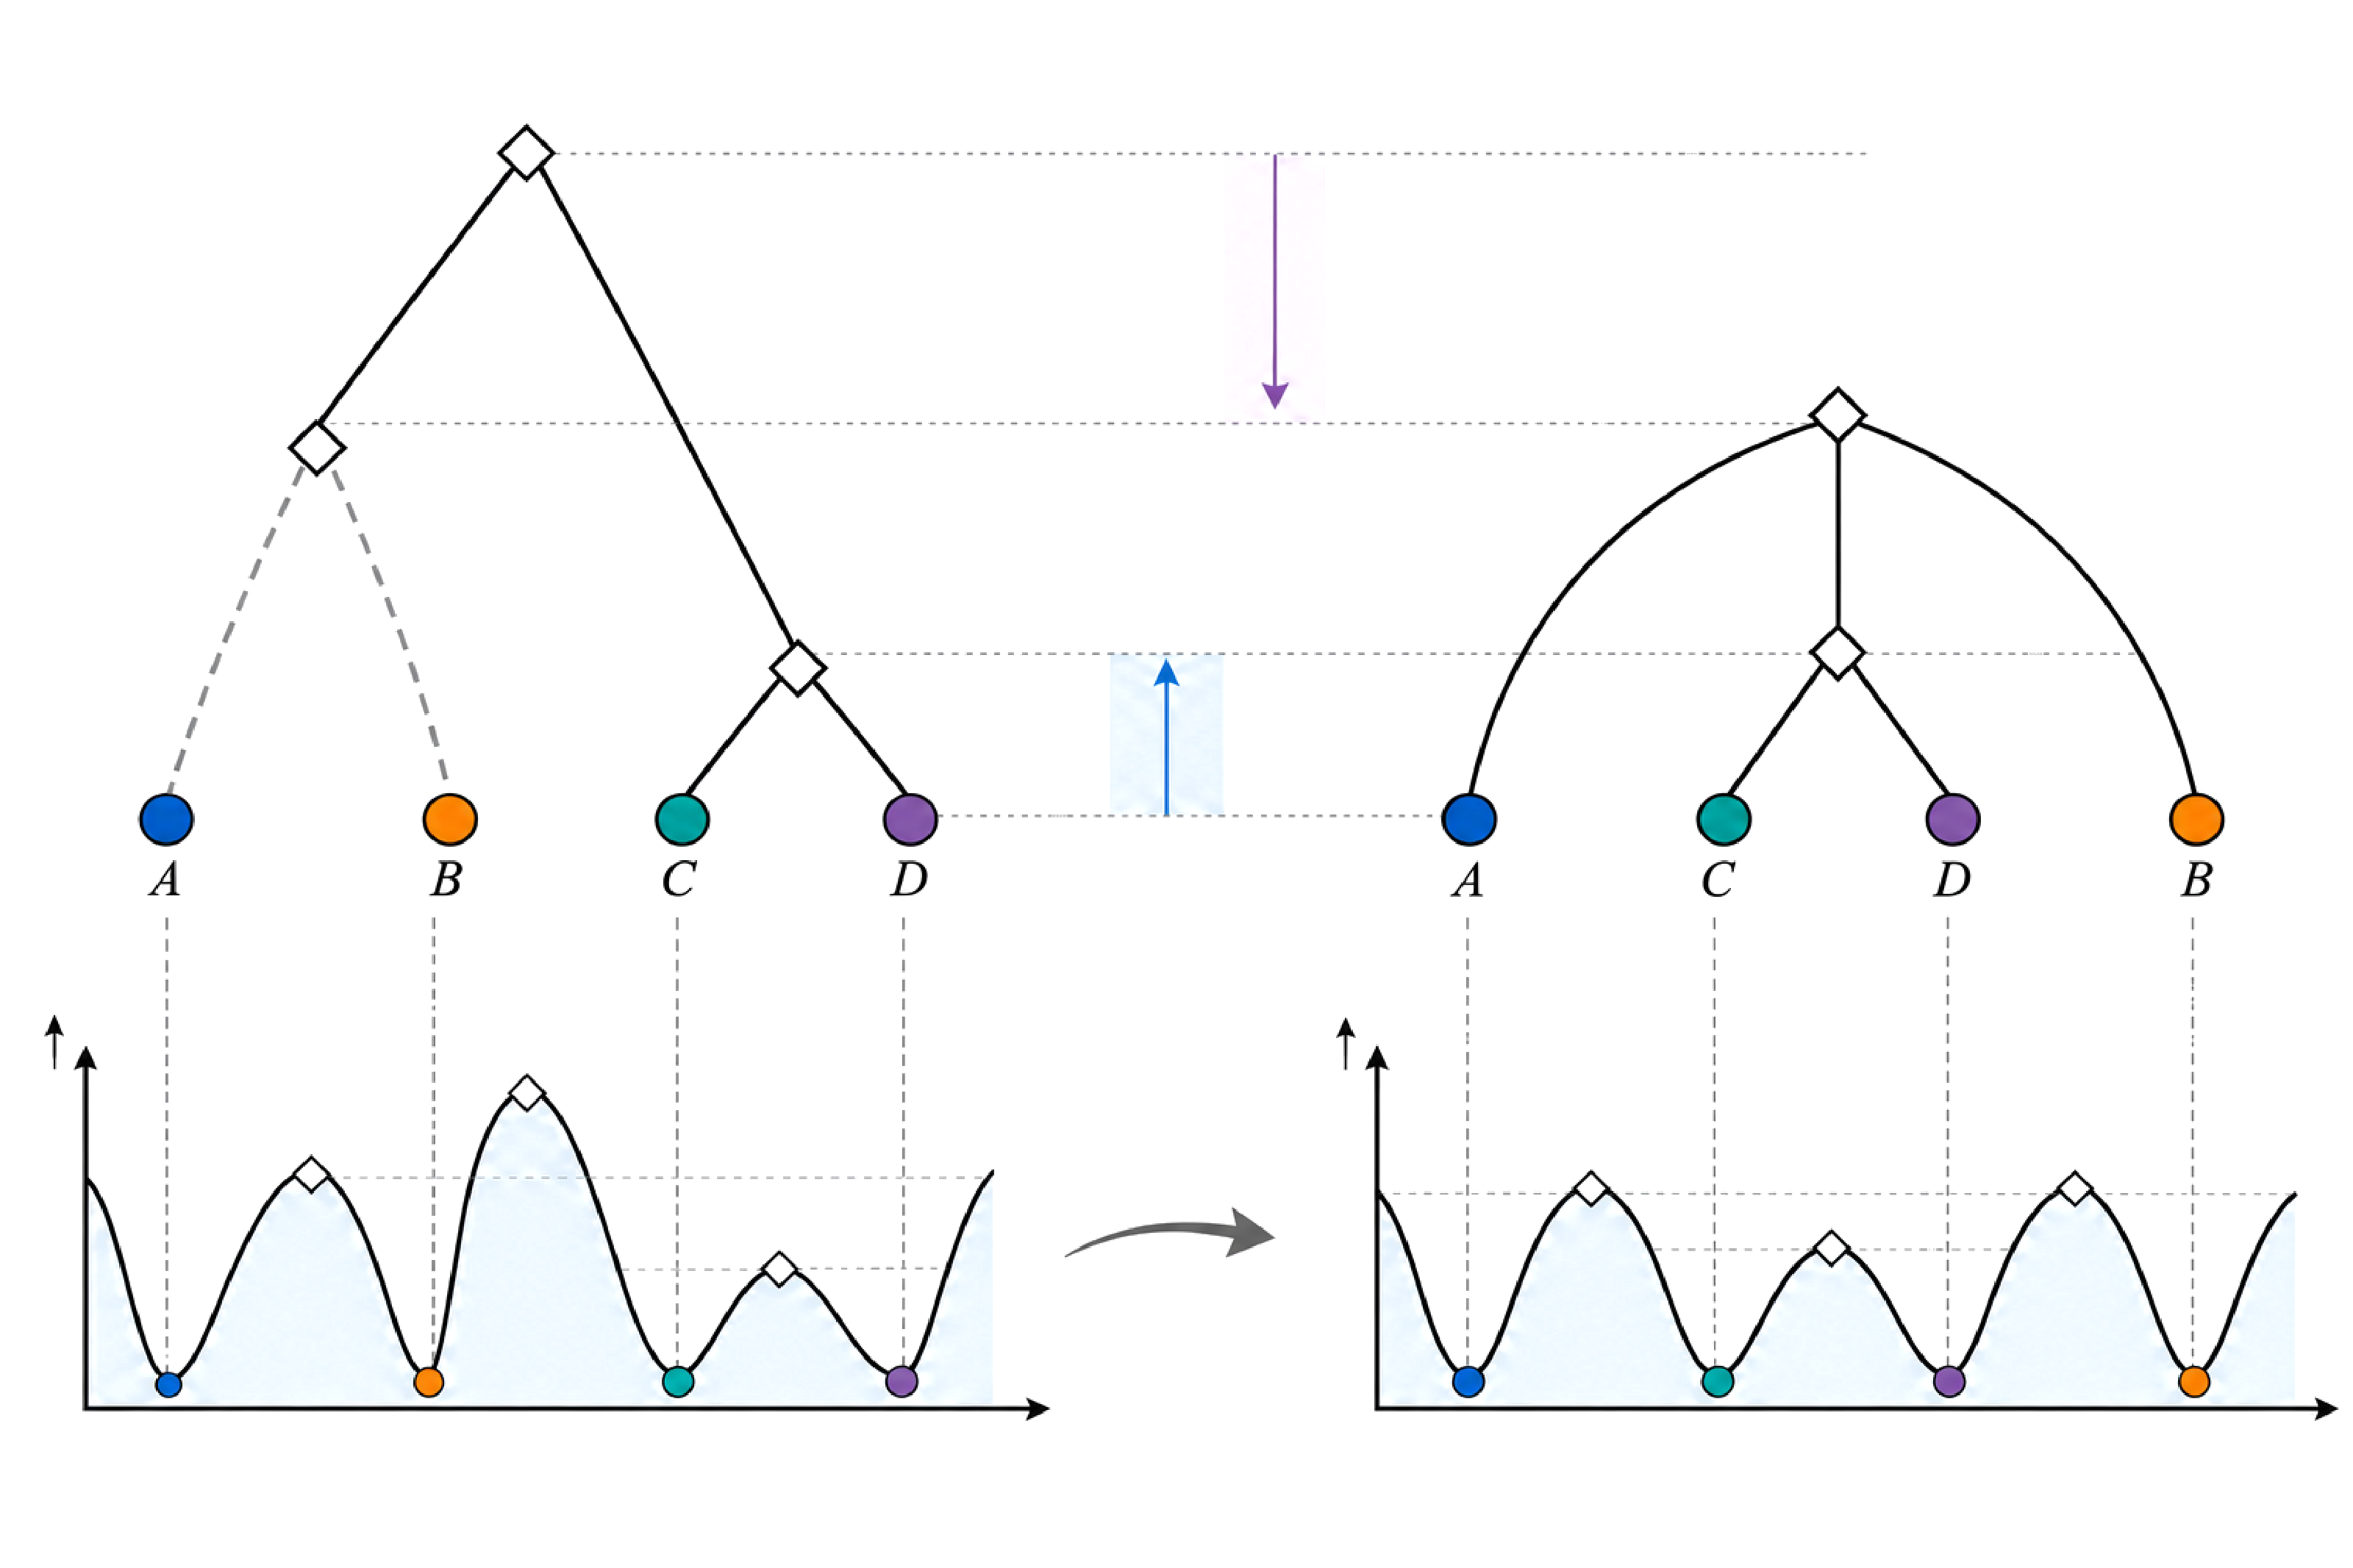
\includegraphics[width=\columnwidth]{../figures/anchor_relaxation_open.pdf}
\caption{Selective relaxation releases the $A,B$ block constraint and admits order $A,C,D,B$ while retaining the $C,D$ grouping. The accompanying profiles illustrate changed merge barriers; source-level guides show the hierarchy changes. Heights are schematic, and candidate orders still require evaluation against the original merge matrix.}
\label{fig:selective_relaxation}
\end{figure}
\section{Experimental Evaluation}\label{sec:experiments}
The evaluation proceeds from overall spatial quality to the effect of topology relaxation and then to map interpretation. Section~\ref{sec:reference-results} compares reference alignment and relative spatial quality on planar and volumetric inputs. Section~\ref{sec:relaxation-results} reports achieved merge errors and position changes under the selected allowances. Case studies then connect these measurements to feature trajectories and spatial snapshots, followed by layout parameters and computational cost.
\begin{table}[t]
\centering
\caption{Volumetric datasets and Balanced-mode parameter settings.}
\label{tab:volume-parameters}
\footnotesize
\setlength{\tabcolsep}{2pt}
\renewcommand{\arraystretch}{0.95}
\begin{tabular}{@{}lcc@{}}
\toprule
Parameter & Cylinder & Tangaroa \\
\midrule
Frames & 102 & 201 \\
Grid & $135\times64\times48$ & $300\times180\times120$ \\
Scalar & $Q$-criterion & Speed $\|\mathbf{v}\|$ \\
Persistence & 2\% per-frame range & 0.2 absolute \\
Reference & $+x$ & $+x$ \\
$\varepsilon$ & 1\% & 33.33\% \\
$L$ & 32768 & 131072 \\
$s_w$ & $2.70668\times10^{-5}$ & 0.40953 \\
Weights & $(0.1,16,0,0.1)$ & $(0,64,0,0)$ \\
$\rho$ & 1 & 1 \\
Gap$/L_{world}$ & $1/300$ & $1/960$ \\
Extra$/L_{world}$ & 0.1 & 0.1 \\
\bottomrule
\end{tabular}
\vspace{2pt}
\begin{minipage}{0.94\columnwidth}\footnotesize Weights are reference, geometry, temporal and eccentricity. $s_w$ is width per support measure (Cylinder voxel counts; Tangaroa physical volume); $L$ is raster length, distinct from the physical canvas extent $L_{world}$. Exact uses zero allowance with the same other parameters as its Balanced counterpart.\end{minipage}
\end{table}

\subsection{Datasets, Baselines and Evaluation Protocol}
Our four planar inputs are Gaussian, Ring, Wildfires and Storms (64, 40, 32 and 744 frames). Raster lengths are 4096, except Ring's original 196 positions. The ST-MTM persistence numbers are tested as per-frame range fractions $p=(0.001,0.001,0.15,0.105)$, or $0.1\%,0.1\%,15\%,10.5\%$; all 880 thresholds were checked~\cite{STMTM:2026}. Gaussian is a three-peak reconstruction, Ring uses the archived generator, Wildfires aggregates FRP into 32 grids, and Storms uses ERA5 anomalies with the archived moving-mean and smoothing convention. Author-processed arrays are unavailable, so these are disclosed local reconstructions, not identical-input reproductions.

PM2.5 adds 744 hourly January 2017 fields on a $160\times144$ interpolation grid. Its shared-input local TMTM, ST-MTM and curve scores are recomputed, with TW $k=1$ on all frames. The PM2.5 mode labelled Balanced uses the 5\% budget fixed from the qualitative case, without validation-set budget selection; both optimization and full-pipeline times are measured without a tree cache. Its SNS and NPE are lowest in this local comparison, while Hilbert has higher TW.

The volumetric inputs are Cylinder (102 frames, $135\times64\times48$, $Q$-criterion)~\cite{Camarri:2005:Cylinder,Weinkauf:SquareCylinder} and Tangaroa (201 frames, $300\times180\times120$, velocity magnitude)~\cite{Popinet:2004:Tangaroa}. Cylinder computes $Q$ from the original $192\times64\times48$ velocity grids before cropping; 2\% persistence uses each frame's scalar range, followed by one fixed sequence scaling of $-Q$. Tangaroa uses speed clipped to $[0,2]$, replaces near-zero values below $10^{-6}$ by the archived inflow value 1, and retains absolute persistence 0.2. These preprocessing choices are shared with the local TMTM adapter. 

For the volumetric comparison, the reference is restricted to the positive Cartesian axes rather than the continuous direction in Section~\ref{sec:reference-model}. The archived offline rule chooses the axis capturing the most squared displacement of matched support centroids, with a minimum-image correction for Cylinder's periodic $z$ coordinate (period 6); both datasets select $+x$. Centroids select the axis only: placement targets remain leaf extrema projected onto that fixed axis and full-domain range. The stored layout configurations are exploratory selections; Table~\ref{tab:volume-parameters} reports their different weights and budgets. 

Within each local dataset, methods share source trees, identities and geometry inputs, and NPE uses one common offline extremum reference and projected range. SNS measures squared scale-normalized stress between support-centroid and anchor distances~\cite{Smelser:2025:Scale,STMTM:2026}; TW measures neighborhoods~\cite{Venna:2001:NP}, with $k=(1,3,5,3)$ and $0<k<n_t/2$. Ineligible frames are omitted. Absolute anchoring uses
\begin{equation}\label{eq:experimental-npe}
\mathrm{NPE}=\frac{1}{T}\sum_t\frac{\max_i|x_i^t-q_i^t|}{L_{world}}.
\end{equation}
TMTM/ST-MTM SNS/TW are quoted from ST-MTM Table~1 (Temporal mode); their NPE is measured with local adapters and shared references. Table~\ref{tab:quantitative-final} distinguishes these sources. Local TW coverage is 64/64, 1/40, 4/32 and 11/744; author coverage is unspecified.

Hilbert and Morton provide sample-domain baselines~\cite{Franke:2021:1DP}. Their grid orientation is fixed ($x$ columns, $y$ rows), with no rotation, reflection or reversal search. Curves use power-of-two padding, discard out-of-domain samples, and map each extremum's full-grid rank to the common canvas at the original raster length. They impose neither merge-tree topology nor finite-width constraints.

\begin{figure*}[t]
\centering
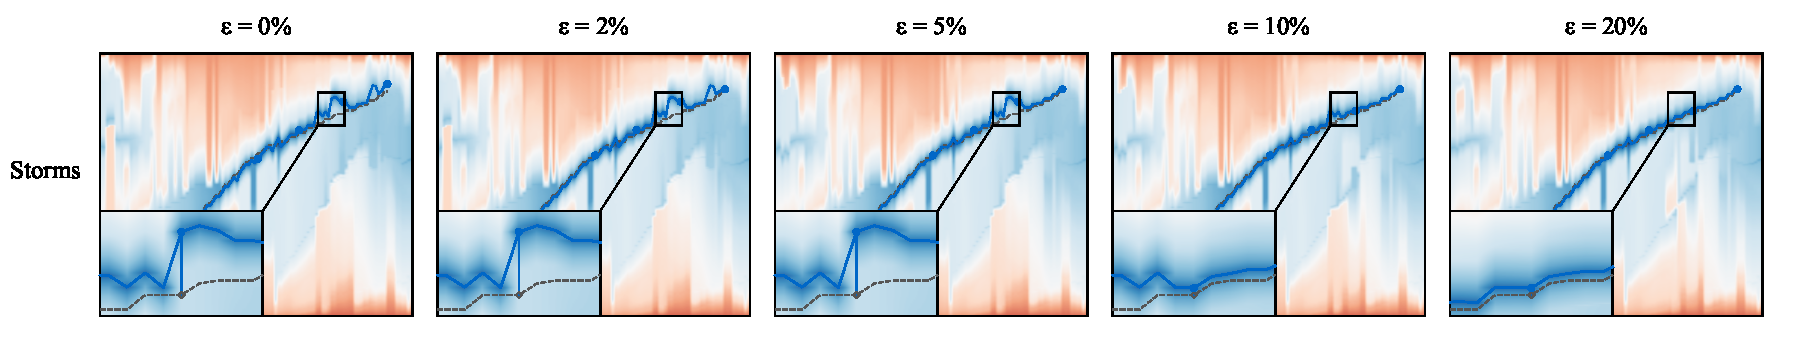
\includegraphics[width=\textwidth]{../figures/anchor_storms_budget_maps.pdf}
\caption{Storms parameter maps and method comparison. AnchorMTM spans exact topology ($\varepsilon=0$) and bounded topology (2, 5, 10 and 20\%), with the original trajectories and common local crops. TMTM and ST-MTM maps use the same scalar fields and augmented trees through local implementations. Spatial awareness and topology budget indicate the respective conceptual improvements. All maps show frames 355--460 with the original blue--orange scale, $[-35,35]$ hPa. }
\label{fig:storms-budget-profiles}
\end{figure*}
\begin{figure}[!t]
\centering
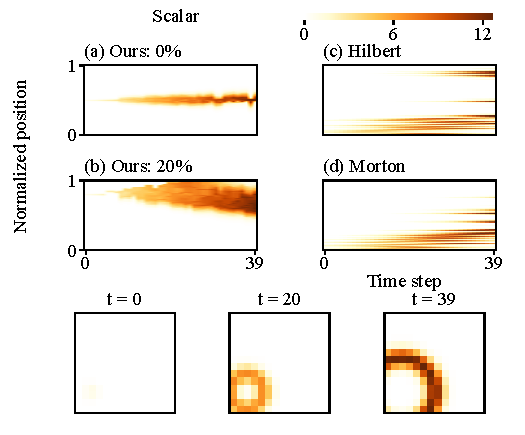
\includegraphics[width=\columnwidth]{../figures/anchor_ring_result.pdf}
\caption{Ring comparison. Top: AnchorMTM at 0, 2, 5, 10 and 20\% topology allowances. Guidance increases jointly with allowance, from neutral central targets to full spatial guidance. Right: supplied Hilbert/Morton reference panels and same-input local TMTM/ST-MTM results. Below: source snapshots at frames 0, 10, 20, 30 and 39. All computed maps use 40 frames and 196 positions; the scalar key applies to computed maps and snapshots. Vertical coordinates denote normalized layout position or curve rank.}
\label{fig:ring-result}
\end{figure}

\begin{figure}[t]
\centering
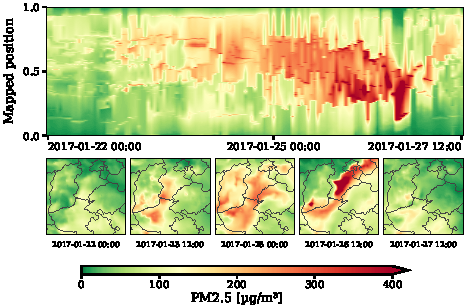
\includegraphics[width=\columnwidth]{../pm25_hourly_20261107/PM25_single_column.pdf}
\caption{Hourly PM2.5 case, January 22 00:00--27 12:00, 2017 (Beijing time). Top: AnchorMTM at $\varepsilon=5\%$. Bottom: five source-field snapshots; labels below the snapshots give date and time. Color above 400 $\mu$g/m$^3$ saturates. The compact rendering retains all 133 hourly samples (both endpoints included); bilinear interpolation is used for display only.}
\label{fig:pm25-hourly}
\end{figure}

\begin{figure*}[t]
\centering
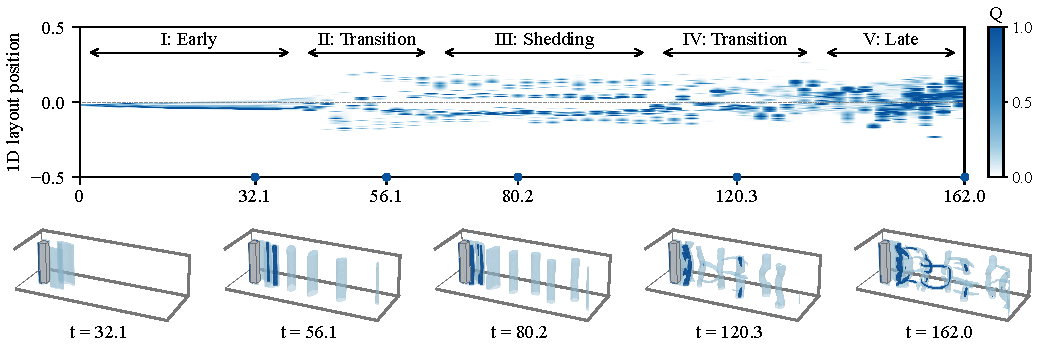
\includegraphics[width=\textwidth]{../figures/anchor_cylinder_centered_blue.pdf}
\caption{Cylinder central-tree variant: the full 102-frame map and source $Q$ isosurfaces at five representative times, with matching time labels, a common camera and a blue scalar scale. $Q=0.2$ is translucent and $Q=1$ marks the core; values above 1 saturate. Map position is not physical $X$; Stages I--V mark early, first-transition, shedding, second-transition and late configurations observed in the map.}
\label{fig:cylinder-centered}
\end{figure*}
\paragraph{Mode selection.}
For the four planar datasets, Exact uses $\varepsilon=0$. Balanced selects a positive budget from 1--10\% (1\% steps) on the first chronological quarter. Among legal reconstructions with attained NMLE$_{\max}\le\varepsilon$, it minimizes
\begin{equation}\label{eq:balanced-validation-score}
J=0.5\,\mathrm{NPE}_{norm}+0.5\,\mathrm{SNS}_{norm}.
\end{equation}
Terms are min--max normalized over legal candidates; constant terms contribute zero. Within 0.01 of the minimum, smaller budgets then attained errors break ties. Budgets are frozen before full runs. Full results include validation frames.

\subsection{Reference Alignment and Relative Spatial Quality}\label{sec:reference-results}
\subsubsection{Planar Results}
Balanced has lower SNS than the published ST-MTM values on all four inputs, but ST-MTM reports higher TW. 

Against fixed Hilbert and Morton curves, Balanced improves SNS and TW on Gaussian, Wildfires and Storms. Ring is an exception: Hilbert achieves SNS 0.1252 and TW 0.9048, versus Balanced's 0.1334 and 0.8571; its TW evidence covers only one eligible frame. Balanced has lower NPE than both curves and both merge-tree adapters on every input. The resulting positions follow the shared spatial reference more closely. Coordinate interpretation also differs across the baselines: traversal coordinates need not represent a physical projection, and relative geometry does not determine an absolute origin.

\subsubsection{Volumetric Results}
\begin{table}[t]
\centering
\caption{Volumetric comparison with a fixed $x$ reference. Bold/underline mark best/second distinct values per dataset; ties share emphasis.}
\label{tab:volume-comparison}
\footnotesize
\setlength{\tabcolsep}{1.2pt}
\renewcommand{\arraystretch}{0.9}
\begin{tabular*}{\columnwidth}{@{\extracolsep{\fill}}lccc lccc@{}}
\toprule
\multirow{2}{*}{Dataset} & \multicolumn{3}{c}{TMTM} & \multicolumn{4}{c}{AnchorMTM (ours)} \\
\cmidrule(lr){2-4}\cmidrule(lr){5-8}
 & SNS$\downarrow$ & TW$\uparrow$ & NPE$\downarrow$ & Mode & SNS$\downarrow$ & TW$\uparrow$ & NPE$\downarrow$ \\
\midrule
\multirow{2}{*}{Cylinder} & \multirow{2}{*}{$0.2956$} & \multirow{2}{*}{$\underline{0.8017}$} & \multirow{2}{*}{$0.4769$} & Exact & $\underline{0.1226}$ & $0.8010$ & $\underline{0.1773}$ \\
 &  &  &  & Balanced & $\mathbf{0.0329}$ & $\mathbf{0.9117}$ & $\mathbf{0.0458}$ \\
\multirow{2}{*}{Tangaroa} & \multirow{2}{*}{$0.5255$} & \multirow{2}{*}{$0.6701$} & \multirow{2}{*}{$0.3866$} & Exact & $\underline{0.1204}$ & $\underline{0.8213}$ & $\underline{0.1285}$ \\
 &  &  &  & Balanced & $\mathbf{0.1124}$ & $\mathbf{0.8408}$ & $\mathbf{0.0653}$ \\
\bottomrule
\end{tabular*}
\vspace{2pt}
\begin{minipage}{\columnwidth}\footnotesize All values are local measurements, including adapted TMTM. TW uses $k=1$, with coverage 102/102 and 201/201. Mode applies only to AnchorMTM. Configurations are frozen exploratory results, not a blind test; settings appear in Table~\ref{tab:volume-parameters}.\end{minipage}
\end{table}

Table~\ref{tab:volume-comparison} follows the planar table's metric order and Exact--Balanced grouping, but compares only with locally adapted TMTM. All three metrics are recomputed over the complete sequences; SNS uses three-dimensional support-centroid distances, TW uses $k=1$ with full frame coverage, and NPE uses extremum targets along the common $x$ axis. Balanced has lower SNS and NPE and higher TW than TMTM on both datasets. Exact and Balanced share the same axis, trees, retained leaf identities and layout weights; only the merge allowance differs. Exact has zero measured fixed-leaf merge error, and both stored Balanced runs pass their declared topology budgets. 

\subsection{Topology Validity and the Position--Topology Trade-off}\label{sec:relaxation-results}
Theorem~\ref{thm:chain} predicts that an allowance can remove ordering conflicts when the relevant accumulated scalar gap is small enough. Exact has zero fixed-leaf merge-matrix error. Balanced attains maximum NMLE of 0, 0.982\%, 4.421\% and 9.985\%, within its allowances; all eight runs pass continuous and raster checks without collapsed anchors. Checks use retained-leaf merge matrices, including diagonal extremum values. Ring requires checked joint integer rounding in 26 Exact and 21 Balanced frames, retaining its 196 positions and continuous order.

Balanced reduces NPE relative to Exact by 17.0\% on Ring, 11.0\% on Wildfires and 65.0\% on Storms. Gaussian is unchanged despite its positive 1\% budget. SNS improves on Ring and Storms but rises from 0.0426 to 0.0447 on Wildfires. 

\subsection{Case Studies of Spatial Coordinate Interpretation}
\subsubsection{Ring: Joint Spatial Guidance and Topology Relaxation}

Figure~\ref{fig:ring-result} shows a joint guidance--topology sweep on Ring: $\varepsilon=0,2,5,10,20\%$ and guidance strength $\alpha=\varepsilon/20\%$. Layout targets interpolate between the canvas midpoint and the fixed $-128.7^\circ$ physical projection: $q_{layout}=(1-\alpha)q_{mid}+\alpha q_{physical}$. Thus stronger guidance moves the reconstructed ring upward through actual optimization. TMTM/ST-MTM maps use the same fields and trees; Hilbert/Morton remain supplied references. Five source snapshots show expansion and strengthening.

\subsubsection{Storms: Feature Positioning Across Topology Budgets}

The upper row of Fig.~\ref{fig:storms-budget-profiles} retains the original five-budget qualitative Storms archive of Fig.~\ref{fig:storms_overview}, separate from main-table preprocessing. The 0, 2 and 5\% layouts overlap locally, while 10 and 20\% move the selected feature toward its fixed reference. The lower row shows TMTM and ST-MTM maps recomputed on these same 744 scalar fields and augmented trees, showing the same event window. TMTM uses overlap-driven temporal subtree alignment in place of anchored placement; ST-MTM uses geometry-based ordering and distance-aware placement with temporal position constraints. The local TMTM implementation handles genuine multiway saddles with equal-level separator copies; the ST-MTM adapter refines them into a stable-ID equal-level binary hierarchy and checks the original leaf LCA matrices. Both baselines use start frame 40 and 8192-position display rasters. 


\subsubsection{PM2.5: Hourly High-Concentration Features}
Figure~\ref{fig:pm25-hourly} adds an exploratory January 2017 case over northern China (110--120 degrees E, 32--41 degrees N), also reported as an additional fixed-configuration row in Tables~\ref{tab:quantitative-final} and~\ref{tab:anchor-parameters-final}. The ChinaVis2021 CAQRA hourly CSV archive provides 744 fields. Linear spatial interpolation produces a $160\times144$ grid without additional smoothing. High concentrations are maxima, handled by join trees of negated concentration, with persistence set to 5\% of each frame's range. The displayed map restores positive concentration. At $\varepsilon=5\%$, all 744 frames pass continuous and raster budget checks; the maximum fixed-leaf NMLE is 4.998\%. The example shows a matched computational peak, not an independently identified pollution parcel.


\subsubsection{Cylinder: Hierarchical Unfolding and Reference Displacement}\label{sec:centered-volume}

The central-tree example is a separate qualitative configuration, excluded from both quantitative tables. Cylinder comprises 102 volumes ($135\times64\times48$) of the $Q$-criterion with 2\% per-frame persistence~\cite{Camarri:2005:Cylinder,Weinkauf:SquareCylinder}. It tests how additional tree guidance changes the map's coordinate interpretation.

The separate Cylinder variant in Fig.~\ref{fig:cylinder-centered} uses the same 102 volumes, retained 2\% persistence trees and a 1\% merge allowance. Full-sample tree coordinates $g_i^t\in[-0.5,0.5]$ add $16\,\mathrm{mean}_i(x_i^t-g_i^t)^2$ to the placement objective; reference, geometry, temporal and eccentricity weights are 1, 1, 0.5 and 0.1. True-$X$ targets retain one fixed domain transform. 

Its fixed tree-compatible order needs a worst-case reference cap of 55.21\%; we explicitly allow 56.21\%, including 1\% slack. Monotone warping of the tree profile through the optimized intervals produces 32768-position rasters. All retained-pair checks yield NMLE$_{max}=0$, within 1\%, including half-pixel position rounding.

The map separates two transition intervals between the early, shedding and late configurations (Fig.~\ref{fig:cylinder-centered}). We mark these visual intervals at approximately $t=40$--65 and $t=105$--135. The five snapshots at $t=32.1$, 56.1, 80.2, 120.3 and 162.0 connect each marked interval to the evolving three-dimensional structures.

Central guidance exposes unfolding but sacrifices anchoring. Frame-balanced mean absolute $X$ error is 21.1\%, 25.5\% and 28.1\% for guidance weights 1, 4 and 16, versus 1.9\% previously. This differs from NPE and pooled mean displacement. Equal-$X$ features may differ in $Y,Z$; their layout separation does not encode depth.

\subsection{Layout Parameters and Computational Cost}
Table~\ref{tab:anchor-parameters-final} lists the four planar Balanced budgets (1, 1, 5 and 10\%) and layout parameters; Table~\ref{tab:volume-parameters} separately lists the volumetric datasets and settings. The planar table reports one uncached Balanced run on Apple M4, with one BLAS/TTK thread, sequential extraction and the default HiGHS scheduler. Optimization includes ordering and placement; total time additionally includes preprocessing, trees, matching/reference estimation, rasterization, I/O and checks. Imports, reporting and metric export are excluded; OS caches may be warm. 

\section{Discussion and Limitations}
The three bounds explain how a hierarchy constrains a spatial axis. Midpoint ordering attains the point-order bound without changing the tree. Finite widths add packing costs, while a merge-error allowance releases selected ordering constraints. This distinction connects the mathematical model to the observed position--topology trade-off.

A fixed reference and relative geometry support different readings of a map. Reference coordinates locate extrema along a chosen direction; pairwise-distance objectives retain relationships among their supports. The lower NPE of the anchored layouts and the higher reported TW of ST-MTM expose this trade-off. The Cylinder example makes it visible within one construction: stronger central-tree guidance reveals unfolding while increasing reference displacement.

The estimated direction depends on overlap-based correspondences. Fast motion and changing supports can interrupt tracks and alter the displacement samples; an analyst-supplied physical direction provides a task-specific alternative. A single projection can also assign the same coordinate to features separated perpendicular to the reference, so spatial snapshots remain useful for resolving those differences.

The order search is heuristic, and finite-width certificates can be loose. These two sources of slack limit how closely a constructed map approaches the smallest feasible displacement. Integer rendering introduces an additional constraint, especially for Ring's 196-position canvas; evaluating the rendered merge matrix accounts for this final step. The reported checks cover retained leaf labels and their diagonal extremum values.

Published SNS/TW and local measurements use different processed inputs and frame coverage. Their values provide context for spatial quality; the shared-input local comparisons provide the direct evidence for reference positioning. Full-sequence statistics include the frames used to select the planar budgets.

\section{Conclusion}
A merge hierarchy imposes measurable conflicts with a spatial reference rather than ruling out a spatial axis. Three algorithm-independent bounds distinguish exact point-order obstruction, finite-width packing and restrictions that remain under a merge-error allowance. AnchorMTM constructs checked temporal maps through reference-aware ordering and capped placement. Existing data comparisons confirm reference alignment and a dataset-dependent response to topology relaxation, and show the accompanying costs in relative spatial fidelity.
% Flush pending floats without forcing an otherwise empty bibliography page.
\FloatBarrier
\begingroup
\interlinepenalty=10000
\bibliographystyle{abbrv-doi-narrow}
\bibliography{../refs}
\endgroup
\end{document}
